\documentclass[11pt,openany]{report}
% =====================================================================
%  RIS project report (Phase 1 + Phase 2), Team 6
%  Build:  pdflatex report_for_RIS  (run twice)
% =====================================================================
\usepackage[T1]{fontenc}
\usepackage[utf8]{inputenc}
\usepackage{lmodern}
\usepackage{microtype}
\usepackage[a4paper,margin=2.2cm,headheight=14pt]{geometry}
\usepackage{amsmath,amssymb,amsthm}
\usepackage{xcolor}
\usepackage{graphicx}
\usepackage{booktabs,array,tabularx,multirow}
\usepackage{enumitem}
\usepackage{float}
\usepackage{caption}
\usepackage{titlesec}
\usepackage{fancyhdr}
\usepackage{pifont}
\usepackage{tcolorbox}
\tcbuselibrary{skins,breakable,theorems}
\usepackage{tikz}
\usetikzlibrary{arrows.meta,positioning,shapes.geometric,shapes.misc,fit,backgrounds,calc,shadows,decorations.pathreplacing,decorations.pathmorphing}
\usepackage{pgfplots}
\pgfplotsset{compat=1.17}
\usepackage[colorlinks=true,linkcolor=deep,citecolor=uavc,urlcolor=uavc]{hyperref}

% ---------------- palette ----------------
\definecolor{deep}{HTML}{0B3954}     % navy    -- TA, overview
\definecolor{uavc}{HTML}{087E8B}     % teal    -- UAVs, C1
\definecolor{vehc}{HTML}{6A4C93}     % violet  -- maths
\definecolor{hoc}{HTML}{E07A1F}      % amber   -- TUAV, C3
\definecolor{tether}{HTML}{B5179E}   % magenta -- C5
\definecolor{quorum}{HTML}{1D5FA8}   % blue    -- C4
\definecolor{bad}{HTML}{C81D25}      % red     -- flaws, attacks
\definecolor{good}{HTML}{2A9D3F}     % green   -- holds, fixed
\definecolor{ink}{HTML}{1F2933}
\definecolor{sun}{HTML}{F4B400}

\color{ink}
\captionsetup{font=small,labelfont={bf,color=deep}}
\setlist{itemsep=2pt,topsep=4pt}
\renewcommand{\arraystretch}{1.18}
\setlength{\parskip}{3pt}

% ---------------- headings ----------------
\titleformat{\chapter}[display]{\bfseries\sffamily\color{deep}}{\large\color{uavc}CHAPTER \thechapter}{4pt}{\huge}
\titlespacing*{\chapter}{0pt}{0pt}{14pt}
\titleformat{\section}{\Large\bfseries\sffamily\color{deep}}{\thesection}{0.8em}{}
\titleformat{\subsection}{\large\bfseries\sffamily\color{uavc}}{\thesubsection}{0.7em}{}
\titleformat{\subsubsection}{\normalsize\bfseries\sffamily\color{ink}}{\thesubsubsection}{0.6em}{}
\pagestyle{fancy}\fancyhf{}
\fancyhead[L]{\small\sffamily\color{deep}CS8.501 Research in Information Security -- Project Report}
\fancyhead[R]{\small\sffamily\color{deep}Team 6}
\fancyfoot[C]{\small\sffamily\thepage}
\renewcommand{\headrulewidth}{0.4pt}

% ---------------- theorem-like environments (numbered per chapter) ----------------
\theoremstyle{plain}
\newtheorem{theorem}{Theorem}[chapter]
\newtheorem{lemma}[theorem]{Lemma}
\newtheorem{corollary}[theorem]{Corollary}
\newtheorem{proposition}[theorem]{Proposition}
\theoremstyle{definition}
\newtheorem{definition}[theorem]{Definition}
\newtheorem{example}[theorem]{Example}
\theoremstyle{remark}
\newtheorem{remark}[theorem]{Remark}
\tcolorboxenvironment{theorem}{enhanced,breakable,colback=vehc!5,colframe=vehc,boxrule=0.6pt,arc=1.5mm,left=4pt,right=4pt}
\tcolorboxenvironment{lemma}{enhanced,breakable,colback=vehc!3,colframe=vehc!70,boxrule=0.5pt,arc=1.5mm,left=4pt,right=4pt}
\tcolorboxenvironment{corollary}{enhanced,breakable,colback=vehc!3,colframe=vehc!70,boxrule=0.5pt,arc=1.5mm,left=4pt,right=4pt}
\tcolorboxenvironment{proposition}{enhanced,breakable,colback=vehc!3,colframe=vehc!70,boxrule=0.5pt,arc=1.5mm,left=4pt,right=4pt}
\tcolorboxenvironment{definition}{enhanced,breakable,colback=deep!4,colframe=deep!70,boxrule=0.5pt,arc=1.5mm,left=4pt,right=4pt}

% ---------------- coloured boxes ----------------
\newtcolorbox{claimbox}[1][]{enhanced,breakable,colback=deep!4,colframe=deep,boxrule=0.6pt,arc=2mm,
  fonttitle=\sffamily\bfseries,title={What the base paper says (quoted)},#1}
\newtcolorbox{flawbox}[1][]{enhanced,breakable,colback=bad!5,colframe=bad,boxrule=0.7pt,arc=2mm,fonttitle=\sffamily\bfseries,#1}
\newtcolorbox{fixbox}[1][]{enhanced,breakable,colback=uavc!6,colframe=uavc,boxrule=0.7pt,arc=2mm,fonttitle=\sffamily\bfseries,#1}
\newtcolorbox{plainbox}[1][]{enhanced,breakable,colback=good!7,colframe=good!80!black,boxrule=0.6pt,arc=2mm,
  fonttitle=\sffamily\bfseries,title={In plain words},#1}
\newtcolorbox{workedbox}[1][]{enhanced,breakable,colback=sun!9,colframe=hoc,boxrule=0.6pt,arc=2mm,fonttitle=\sffamily\bfseries,#1}
\newtcolorbox{keybox}[1][]{enhanced,breakable,colback=deep!5,colframe=deep,boxrule=0.6pt,arc=2mm,
  fonttitle=\sffamily\bfseries,title={Key idea},#1}
\newtcolorbox{limitbox}[1][]{enhanced,breakable,colback=black!3,colframe=black!55,boxrule=0.6pt,arc=2mm,
  fonttitle=\sffamily\bfseries,title={Scope and honest limits},#1}
\newtcolorbox{algobox}[2][]{enhanced,breakable,colback=white,colframe=vehc,boxrule=0.8pt,arc=2mm,
  fonttitle=\sffamily\bfseries,coltitle=white,colbacktitle=vehc,title={#2},#1}
\newcounter{algo}[chapter]
\renewcommand{\thealgo}{\thechapter.\arabic{algo}}
\newenvironment{algorithm}[1]{\refstepcounter{algo}\begin{algobox}{Algorithm \thealgo: \;#1}}{\end{algobox}}
\newtcolorbox{stepbox}[2]{enhanced,breakable,colback=white,colframe=#1,boxrule=0.8pt,arc=2mm,
  fonttitle=\sffamily\bfseries,coltitle=white,colbacktitle=#1,title={#2}}

% ---------------- notation ----------------
\newcommand{\TA}{\mathsf{TA}}
\newcommand{\U}{\mathcal{U}}
\newcommand{\Adv}{\mathcal{A}}
\newcommand{\G}{\mathbb{G}}
\newcommand{\Zq}{\mathbb{Z}_q^{*}}
\newcommand{\Ppub}{P_{\mathrm{pub}}}
\newcommand{\Tpub}{T_{\mathrm{pub}}}
\newcommand{\PID}{\mathit{PID}}
\newcommand{\RID}{\mathit{RID}}
\newcommand{\ID}{\mathit{ID}}
\newcommand{\pk}{\mathit{pk}}
\newcommand{\sk}{\mathit{sk}}
\newcommand{\ep}{\mathit{ep}}
\newcommand{\ts}{\mathit{ts}}
\newcommand{\GK}{\mathit{GK}}
\newcommand{\Enc}{\mathsf{Enc}}
\newcommand{\KDF}{\mathsf{KDF}}
\newcommand{\Hz}{H_0}
\newcommand{\Ho}{H_1}
\newcommand{\Ht}{H_2}
\newcommand{\Hd}{H_3}
\newcommand{\BH}{\mathsf{H}_1}
\newcommand{\MAC}{\mathsf{MAC}}
\newcommand{\Tk}{\mathit{Tk}}
\newcommand{\hk}{\mathit{hk}}
\newcommand{\M}{\mathcal{M}}
\newcommand{\Ta}{\mathcal{T}_a}
\newcommand{\Tb}{\mathcal{T}_b}
\newcommand{\cat}{\,\|\,}
\newcommand{\yes}{\textcolor{good}{\ding{51}}}
\newcommand{\no}{\textcolor{bad}{\ding{55}}}
\newcommand{\steplabel}[2]{\textcolor{#1}{\textsf{\textbf{#2}}}}
\newcommand{\badge}[2]{\tikz[baseline=(t.base)]\node[fill=#1,text=white,rounded corners=2pt,inner sep=2pt,font=\scriptsize\sffamily\bfseries](t){#2};}

% ---------------- TikZ styles and icons ----------------
\tikzset{
  ent/.style={draw=#1,fill=#1!12,very thick,rounded corners=3pt,minimum width=2.3cm,minimum height=0.9cm,
              align=center,font=\sffamily\small\bfseries,drop shadow={opacity=0.15}},
  ent/.default=deep,
  msg/.style={-{Stealth[length=2.6mm]},thick,draw=#1},
  msg/.default=ink,
  lbl/.style={font=\scriptsize\sffamily,fill=white,inner sep=1.5pt,align=center},
  life/.style={draw=black!30,dashed},
  act/.style={draw=#1,fill=#1!8,rounded corners=2pt,font=\scriptsize\sffamily,align=left,inner sep=3pt},
  tier/.style={draw=#1,fill=#1!5,rounded corners=6pt,dashed,thick},
  card/.style={draw=#1,fill=#1!10,very thick,rounded corners=4pt,align=center,font=\sffamily\small,inner sep=5pt,
               drop shadow={opacity=0.15}},
  % flowchart shapes
  fstart/.style={draw=#1,fill=#1!15,thick,rounded corners=9pt,align=center,font=\sffamily\scriptsize\bfseries,inner sep=5pt,minimum height=0.8cm},
  fproc/.style={draw=#1,fill=#1!7,thick,rounded corners=2pt,align=center,font=\sffamily\scriptsize,inner sep=4pt,minimum height=0.8cm},
  fdec/.style={draw=#1,fill=#1!10,thick,diamond,aspect=2.2,align=center,font=\sffamily\scriptsize,inner sep=1pt},
  fio/.style={draw=#1,fill=#1!8,thick,trapezium,trapezium left angle=72,trapezium right angle=108,align=center,font=\sffamily\scriptsize,inner sep=3pt,minimum height=0.8cm},
  flow/.style={-{Stealth[length=2.2mm]},thick,draw=black!65},
  pics/drone/.style={code={
    \draw[line width=1.3pt] (-0.32,-0.32) -- (0.32,0.32) (-0.32,0.32) -- (0.32,-0.32);
    \foreach \x/\y in {-0.32/-0.32,0.32/0.32,-0.32/0.32,0.32/-0.32}{\draw[line width=1pt,fill=white] (\x,\y) circle (0.15);}
    \fill (0,0) circle (0.11);}},
  pics/truck/.style={code={
    \draw[thick,fill=white] (-0.62,-0.14) rectangle (0.22,0.36);
    \draw[thick,fill=white] (0.22,-0.14) -- (0.22,0.22) -- (0.46,0.22) -- (0.6,0.04) -- (0.6,-0.14) -- cycle;
    \fill (-0.36,-0.2) circle (0.1) (0.38,-0.2) circle (0.1);}},
  pics/sat/.style={code={
    \draw[thick,fill=white] (-0.14,-0.14) rectangle (0.14,0.14);
    \draw[thick,fill=white] (-0.6,-0.09) rectangle (-0.22,0.09);
    \draw[thick,fill=white] (0.22,-0.09) rectangle (0.6,0.09);
    \draw[thick] (-0.22,0) -- (-0.14,0) (0.14,0) -- (0.22,0);}},
  pics/ta/.style={code={
    \draw[thick,fill=white] (-0.45,-0.35) rectangle (0.45,0.14);
    \draw[thick,fill=white] (-0.56,0.14) -- (0,0.44) -- (0.56,0.14) -- cycle;
    \foreach \x in {-0.3,-0.1,0.1,0.3}{\draw[thick] (\x,-0.3) -- (\x,0.09);}}},
  pics/car/.style={code={
    \draw[thick,fill=white,rounded corners=2pt] (-0.45,-0.1) rectangle (0.45,0.15);
    \draw[thick,fill=white,rounded corners=2pt] (-0.25,0.15) rectangle (0.22,0.33);
    \fill (-0.25,-0.14) circle (0.08) (0.25,-0.14) circle (0.08);}},
  pics/chip/.style={code={
    \draw[thick,fill=white,rounded corners=1pt] (-0.22,-0.22) rectangle (0.22,0.22);
    \foreach \t in {-0.12,0,0.12}{\draw[thick] (\t,0.22) -- (\t,0.32) (\t,-0.22) -- (\t,-0.32) (0.22,\t) -- (0.32,\t) (-0.22,\t) -- (-0.32,\t);}
    \node[font=\tiny\sffamily\bfseries] at (0,0) {g};}},
  pics/tower/.style={code={
    \draw[thick] (-0.25,-0.45) -- (0,0.4) -- (0.25,-0.45) (-0.16,-0.15) -- (0.16,-0.15) (-0.09,0.1) -- (0.09,0.1);
    \draw[thick] (-0.12,0.5) arc (150:30:0.14) (-0.2,0.58) arc (150:30:0.23);}},
}

% ---------------- part divider ----------------
\newcommand{\partpage}[4]{% #1 colour, #2 label, #3 title, #4 one-line summary
  \cleardoublepage\thispagestyle{empty}
  \addcontentsline{toc}{part}{#2\quad #3}
  \begin{tikzpicture}[remember picture,overlay]
    \fill[#1] (current page.north west) rectangle ([yshift=-11cm]current page.north east);
    \node[anchor=west,text=white,font=\sffamily\bfseries\fontsize{54}{54}\selectfont] at ([xshift=2cm,yshift=-4.2cm]current page.north west) {#2};
    \node[anchor=west,text=white,font=\sffamily\bfseries\huge,text width=16cm] at ([xshift=2cm,yshift=-7cm]current page.north west) {#3};
    \node[anchor=west,text=#1!60!black,font=\sffamily\Large,text width=16cm] at ([xshift=2cm,yshift=-13cm]current page.north west) {#4};
  \end{tikzpicture}
  \clearpage}

\graphicspath{{figs/}}

\begin{document}
% ============================== title page (course template) ==============================
\begin{titlepage}
\centering
\vspace*{1.2cm}
{\fontsize{23}{28}\selectfont\bfseries Cutting the Cord: Trust Without the TA\par}
\vspace{0.3cm}
{\Large Security Analysis and Improvements of a TUAV-Assisted\\ Key Management Scheme for Infrastructure-Less IoVs\par}
\vspace{0.6cm}
{\large CS8.501 -- Research in Information Security\par}
{\large Project Report\par}
\vspace{1.0cm}
{\large Submitted by: Team 6\par}
\vspace{0.2cm}
{\large Swaraj Kumar\par}
{\large Hritik Ranjan\par}
{\large Harsh Raj\par}
\vspace{0.3cm}
{\large Department: Computer Science and Information Security\par}
\vspace{0.6cm}
{\large Date of Submission: November 17, 2026\par}
\vspace{1.4cm}

\includegraphics[width=0.62\linewidth]{iiith_logo.png}\par
\vfill
{\Large International Institute of Information Technology, Hyderabad\par}
\vspace{0.8cm}
\end{titlepage}

% ============================== abstract ==============================
\chapter*{Abstract}
\addcontentsline{toc}{chapter}{Abstract}
This report presents our course project on the paper ``Secure and Efficient Authenticated Key Management Scheme for UAV-Assisted
Infrastructure-Less IoVs'' by H.~Tan, W.~Zheng and P.~Vijayakumar (IEEE T-ITS, 2023)~\cite{tan2023}. The paper replaces broken roadside units in a
disaster area with a \emph{tethered} UAV (TUAV) that is powered by a fire truck (ECRV), and uses a trusted authority (TA), reached by satellite, to
authenticate a group of UAVs and give them a group key built with the Chinese Remainder Theorem (CRT).

We first study the paper in detail: its motivation, system model, the five protocol phases (IS, US, GA, GD, DU), and its security and
performance claims. We then check those claims against the paper's own equations. We prove three weaknesses: the TA can sign as any
UAV (F1), the CRT group key leaks every member's key -- even to a passive outsider who compares two broadcasts (F2), and one leaked long-term secret
opens all past group keys (F3). We then propose four contributions: authentication with the TA offline and a separately sealed key for every member
(C1), handover between TUAVs (C2), voting out a compromised TUAV (C3) and splitting the TUAV's key across its tether (C4). Each result comes with a
theorem, a worked example and a diagram.

\tableofcontents
\listoffigures

% ============================== introduction ==============================
% =====================================================================
\chapter{Introduction}\label{ch:intro}
% =====================================================================
\section{About this project}
This is the project report for the course \textbf{CS8.501 -- Research in Information Security}. The project is based on one research paper:
\begin{quote}
H.~Tan, W.~Zheng and P.~Vijayakumar, ``Secure and Efficient Authenticated Key Management Scheme for UAV-Assisted Infrastructure-Less IoVs,''
\emph{IEEE Transactions on Intelligent Transportation Systems}, vol.~24, no.~6, pp.~6389--6400, June 2023~\cite{tan2023}.
\end{quote}

\section{Problem statement}
After an earthquake or a flood, roadside units (RSUs) and mobile towers often stop working. Rescue vehicles still need to communicate, and the
communication must be authenticated and confidential. The base paper uses a \textbf{tethered UAV (TUAV)}, a drone powered through a cable by an
emergency vehicle (ECRV), as a flying base station. Battery UAVs extend its coverage, and a trusted authority (TA) is reached over a satellite link.
The TA authenticates a group of UAVs, and the TUAV gives them a group key.

Our problem has two parts: (i) check whether the scheme really gives the security properties it claims, and (ii) where it does not, design
improvements that keep the system working securely in a disaster area.

\section{Summary of our work}
\begin{center}
\begin{tabularx}{\linewidth}{@{}p{3.2cm} X@{}}
\toprule
\textbf{Part} & \textbf{What we did}\\
\midrule
Study of the paper & We studied the base paper in detail: the problem it solves, its system model, the protocol step by step, and its security and
performance claims (Chapters~\ref{ch:bg}--\ref{ch:p1analysis}).\\
Analysis and design & We checked every security claim against the paper's own equations, proved three weaknesses (F1--F3), and designed four
contributions (C1--C4) that fix them and cover situations the paper does not handle (Chapters~\ref{ch:p2overview}--\ref{ch:concl}).\\
\bottomrule
\end{tabularx}
\end{center}

\section{Team and individual contributions}
All three members studied the base paper, took part in the discussions and reviewed the final report. The main responsibilities were:
\begin{center}
\begin{tabularx}{\linewidth}{@{}l l X@{}}
\toprule
\textbf{Member} & \textbf{Roll number} & \textbf{Main responsibilities}\\
\midrule
Swaraj Kumar & 2025202016 & study of the paper's motivation, system model and protocol; overall framework of our design; compiling the report\\
Hritik Ranjan & 2025202031 & mathematical analysis of the three weaknesses (F1, F2, F3); construction of C1 and its security theorems\\
Harsh Raj & 2025202005 & design and security analysis of C2, C3 and C4; the hardening study A1--A7; security comparison and results\\
\bottomrule
\end{tabularx}
\end{center}

\section{Organisation of the report}
Chapter~\ref{ch:bg} gives the mathematical background. Chapter~\ref{ch:p1paper} summarises the paper's motivation, contributions and related work.
Chapter~\ref{ch:base} describes the protocol, and Chapter~\ref{ch:p1analysis} summarises the paper's own security and performance analysis.
Chapter~\ref{ch:p2overview} gives an overview of our results. Chapters~\ref{ch:f1}--\ref{ch:f3} prove the three weaknesses,
Chapters~\ref{ch:c1}--\ref{ch:hard} present our contributions, and Chapters~\ref{ch:results}--\ref{ch:concl} compare, discuss and conclude.


% ============================== the base paper ==============================

% =====================================================================
\chapter{Mathematical background}\label{ch:bg}
% =====================================================================
This chapter collects every tool used later. Where a result has a standard name we use it, so a reader can look it up.

\section{Notation}
\begin{center}
\small
\begin{tabularx}{\linewidth}{@{}l X@{}}
\toprule
\textbf{Symbol} & \textbf{Meaning}\\
\midrule
$\G_1,\G_2,\ \hat e,\ P,\ q$ & base paper: additive group $\G_1$ and multiplicative group $\G_2$ of prime order $q$, pairing $\hat e:\G_1\times\G_1\to\G_2$, generator $P$\\
$\langle id_i,s_i\rangle$ & base paper: true identity and long-term secret of UAV $i$, issued and \emph{stored} by the TA (IS2)\\
$r_i,\ \xi_i=h_1(r_i)$ & base paper: UAV's random value and its hash; $\xi_i$ is sent in the clear (US3)\\
$\ID_i,\ \upsilon_i,\ \Gamma_i$ & base paper: session identity, check value and credential of UAV $i$ (US1--US2)\\
$\sigma_i=h_1(s_i\xi_i)P$ & base paper: ``decrypting key'' of UAV $i$, used as a CRT modulus (GD1)\\
$\Lambda(x)=\sum_{k=0}^{n}a_kx^k$ & base paper: broadcast polynomial; $\{a_k\}$ is the public coefficient set (GD2, GD4)\\
$\kappa_{tu}$ & base paper: group key\\
\midrule
$\G,\ P,\ q$ & our design: a prime-order elliptic-curve group (no pairing needed)\\
$s,\ \Ppub=sP$ & our design: TA master key and public key (used only before the mission)\\
$x,\ d,\ \sk=x+d,\ \pk$ & our design: user secret, partial key from the TA, full signing key, public key\\
$e,\ E=eP$ & ephemeral Diffie--Hellman values, erased after use\\
$\GK,\ \nu$ & our group key and its version number\\
$\KDF,\ \Enc$ & key-derivation function (e.g.\ HKDF~\cite{hkdf}) and authenticated encryption with associated data (AEAD~\cite{aead})\\
$a,\ g$ & C4: the drone's share and the ECRV chip's share of the TUAV key, $\sk=a+g$\\
\bottomrule
\end{tabularx}
\end{center}

\section{Groups, pairings and hard problems}
The base paper uses a symmetric pairing $\hat e:\G_1\times\G_1\to\G_2$ with \textbf{bilinearity}
\[
\hat e(aP,bQ)=\hat e(P,Q)^{ab},\qquad \hat e(Q+R,P)=\hat e(Q,P)\,\hat e(R,P),
\]
non-degeneracy and efficient computability (paper, Section~III-A). Security rests on two problems, defined in the paper as Definitions~1 and~2.

\begin{definition}[ECDLP]
Given $P$ and $Q=aP$, find $a$. The problem is hard if every probabilistic polynomial-time (PPT) algorithm succeeds with negligible probability.
\end{definition}
\begin{definition}[CDH]
Given $P$, $aP$ and $bP$ for unknown $a,b$, compute $abP$. Hard if every PPT algorithm succeeds with negligible probability.
\end{definition}
\noindent A CDH \emph{instance} is only hard if $a$ and $b$ are unknown; if $b$ is public, anyone computes $abP=b\cdot(aP)$.

\section{Four named theorems we use}
\begin{theorem}[Chinese Remainder Theorem]\label{thm:crt}
Let $m_1,\dots,m_n$ be pairwise coprime positive integers and $M=\prod_im_i$. For any $c_1,\dots,c_n$ there is exactly one $X\in[0,M)$ with
$X\equiv c_i\pmod{m_i}$ for all $i$, namely $X=\sum_i c_i\,\omega_i\varphi_i \bmod M$, where $\omega_i=M/m_i$ and $\varphi_i\equiv\omega_i^{-1}\pmod{m_i}$.
\end{theorem}
The base paper uses the special case $c_1=\dots=c_n=\kappa_{tu}$: the number $\kappa_{tu}\sum_i\omega_i\varphi_i$ leaves remainder $\kappa_{tu}$ modulo every
$\sigma_i$ (Lemma~\ref{lem:gd6}).

\begin{theorem}[Vieta's formulas]\label{thm:vieta}
If $p(x)=\prod_{i=1}^{n}(x-\sigma_i)=x^n+c_{n-1}x^{n-1}+\dots+c_1x+c_0$, then $c_{n-k}=(-1)^k e_k(\sigma_1,\dots,\sigma_n)$, where $e_k$ is the $k$-th
elementary symmetric polynomial. In particular
\[
c_{n-1}=-(\sigma_1+\sigma_2+\dots+\sigma_n),\qquad c_0=(-1)^n\sigma_1\sigma_2\cdots\sigma_n .
\]
\end{theorem}

\begin{theorem}[Rational Root Theorem]\label{thm:rrt}
If a polynomial with integer coefficients has a rational root $u/v$ in lowest terms, then $u$ divides the constant coefficient and $v$ divides the leading
coefficient. For a monic polynomial every rational root is an integer.
\end{theorem}

\begin{proposition}[Integer roots are easy to find]\label{prop:roots}
All integer roots of an integer polynomial of degree $n$ with $B$-bit coefficients can be found in time polynomial in $n$ and $B$ -- for example by
factoring with the LLL algorithm~\cite{lll}, or by Cantor--Zassenhaus factoring modulo a prime followed by Hensel lifting~\cite{cz}. When all roots are
real and distinct (our case), real-root isolation followed by bisection finds each root of size at most $2^{160}$ in about $160$ halving steps.
\end{proposition}
\noindent So recovering the $\sigma_i$ from a known product polynomial is \textbf{not} a brute-force search; it is a routine computation.

\section{Signatures, forking and batch verification}
\begin{definition}[Schnorr-type signature~\cite{schnorr}]
Key pair $(\sk,\ \pk=\sk\cdot P)$. To sign $m$: pick random $r$, set $R=rP$, $c=H(m\cat R\cat\dots)$, $v=r+c\cdot\sk\bmod q$; output $(R,v)$.
To verify: check $vP\overset{?}{=}R+c\cdot\pk$.
\end{definition}

\begin{lemma}[General Forking Lemma~\cite{forking,bnforking}, informal]\label{lem:fork}
If an adversary making at most $q_H$ hash queries outputs a valid signature with probability $\varepsilon$, then re-running it with the same random tape
but fresh hash answers from the critical query yields two valid signatures $(R,v)$, $(R,v')$ with the same $R$ and different challenges $c\neq c'$ with
probability at least about $\varepsilon^2/q_H$. From $vP=R+c\,\pk$ and $v'P=R+c'\,\pk$ one extracts $\sk=(v-v')(c-c')^{-1}$, solving the ECDLP for $\pk$.
\end{lemma}

\begin{lemma}[Small-Exponent Test, Bellare--Garay--Rabin~\cite{bgr}]\label{lem:bgr}
Let $\Delta_1,\dots,\Delta_n\in\G$ (prime order $q$) and let $\lambda_1,\dots,\lambda_n$ be chosen uniformly from $\{1,\dots,2^\ell\}$ with $2^\ell<q$.
If some $\Delta_j\neq 0$, then $\Pr\big[\sum_i\lambda_i\Delta_i=0\big]\le 2^{-\ell}$.
\end{lemma}
\begin{proof}
Write $\Delta_i=\delta_iP$ with $\delta_j\neq0$. The sum is zero iff $\sum_i\lambda_i\delta_i\equiv0\pmod q$. Fix every $\lambda_i$ with $i\neq j$; then the
equation holds for exactly one value of $\lambda_j$ modulo $q$, namely $-\delta_j^{-1}\sum_{i\ne j}\lambda_i\delta_i$. Since $\lambda_j$ is uniform over
$2^\ell<q$ values, it hits that value with probability at most $2^{-\ell}$.
\end{proof}
\noindent Applied with $\Delta_i=v_iP-R_i-c_i\pk_i$ (the ``error'' of signature $i$), the test accepts a batch containing an invalid signature with
probability at most $2^{-\ell}$; we use $\ell=64$. Without weights ($\lambda_i=1$), errors $+\Delta$ and $-\Delta$ cancel.

\section{Security properties we test}
\begin{definition}[Key-escrow resilience and Girault's trust levels~\cite{girault}]
A scheme is \emph{key-escrow resilient} if the authority that issues credentials cannot produce valid signatures in a user's name. Girault grades
authorities as: \textbf{level 1} -- it knows users' secret keys and can impersonate without trace; \textbf{level 2} -- it does not know them, but can
impersonate by issuing a false credential (a second public key); \textbf{level 3} -- any such false credential can be proven.
\end{definition}

\begin{definition}[Non-repudiation]
A sender cannot later deny a message it signed; equivalently, nobody else (including the authority) could have produced that signature.
\end{definition}

\begin{definition}[Group-key secrecy, revocation and backward secrecy]
For a sequence of group keys $\kappa^{(1)},\kappa^{(2)},\dots$: \emph{secrecy} -- no non-member learns a current key; \emph{revocation} (forward group
secrecy) -- a member removed before epoch $t$ learns nothing about $\kappa^{(t)},\kappa^{(t+1)},\dots$; \emph{backward secrecy} -- a member that joins in
epoch $t$ learns nothing about $\kappa^{(1)},\dots,\kappa^{(t-1)}$.
\end{definition}

\begin{definition}[Forward secrecy]
Session (or group) keys established before a long-term secret is compromised remain secret after the compromise.
\end{definition}

\section{Adversary models}
\begin{center}
\small
\begin{tabularx}{\linewidth}{@{}l X l@{}}
\toprule
\textbf{Adversary} & \textbf{Capabilities} & \textbf{Used in}\\
\midrule
Passive outsider & records every radio message (Dolev--Yao eavesdropper~\cite{dolevyao}); never registered & F2(c)\\
Active outsider & also injects, replays, drops and modifies messages & C1, C2\\
Insider (current or former member) & knows its own secrets and everything it ever received & F2(a), F2(b)\\
Malicious or breached TA & knows everything the TA stores ($\langle id_i,s_i\rangle$ in the base paper; $s$, $d_i$ in ours) & F1, C1\\
Long-term-key thief & obtains $s_i$ (e.g.\ from a captured UAV) later in time & F3, C1\\
Captured TUAV & has the drone's full memory but no longer the tether & C4\\
Compromised TUAV & software takeover while still tethered & C3, A1--A7\\
\bottomrule
\end{tabularx}
\end{center}

% =====================================================================
\chapter{The base paper at a glance}\label{ch:p1paper}
% =====================================================================
\section{Motivation given by the paper}
The paper starts from three observations (Section~I of~\cite{tan2023}):
\begin{enumerate}[leftmargin=*]
\item Vehicle networks (IoVs) normally rely on roadside units (RSUs) at the edge. Existing authentication schemes assume these RSUs work. In a disaster
they may not, and then vehicle-to-infrastructure (V2I) communication fails.
\item Modern roads are three-dimensional (bridges, flyovers, tunnels), so flat ground coverage is not enough. Satellites have high latency and cost, so
the paper prefers UAVs as an aerial extension of the network.
\item Ordinary UAVs fly for less than an hour on battery. A \textbf{tethered UAV} gets power through a cable from a ground vehicle, so it can hover for a
long time and act as a mobile base station and edge server.
\end{enumerate}

\begin{figure}[H]
\centering
\resizebox{0.92\linewidth}{!}{%
\begin{tikzpicture}[font=\sffamily\small]
  \node[card=deep,text width=5.6cm,minimum height=4.0cm] (a) at (0,0) {};
  \node[font=\sffamily\bfseries,text=deep] at (0,1.65) {Normal IoV};
  \pic[color=deep,scale=1.1] at (0,0.35) {tower};
  \foreach \x in {-1.6,-0.5,0.6,1.7}{\pic[color=vehc,scale=0.8] at (\x,-0.9) {car};}
  \node[font=\scriptsize\sffamily,text=deep] at (0,-1.6) {vehicles talk through the RSU};
  \node[card=bad,text width=5.6cm,minimum height=4.0cm] (b) at (7,0) {};
  \node[font=\sffamily\bfseries,text=bad] at (7,1.65) {After a disaster};
  \pic[color=black!45,scale=1.1] at (7,0.35) {tower};
  \draw[bad,line width=2pt] (6.6,-0.15) -- (7.4,0.85) (6.6,0.85) -- (7.4,-0.15);
  \foreach \x in {5.4,6.5,7.6,8.7}{\pic[color=vehc,scale=0.8] at (\x,-0.9) {car};}
  \node[font=\scriptsize\sffamily,text=bad] at (7,-1.6) {RSU down: no V2I link};
  \node[card=hoc,text width=5.6cm,minimum height=4.0cm] (c) at (14,0) {};
  \node[font=\sffamily\bfseries,text=hoc] at (14,1.65) {The paper's idea};
  \pic[color=hoc,scale=0.9] at (13.3,0.75) {drone};
  \draw[tether,line width=1.4pt] (13.3,0.4) -- (13.3,-0.55);
  \pic[color=hoc,scale=0.9] at (13.3,-0.8) {truck};
  \pic[color=uavc,scale=0.6] at (14.6,0.8) {drone};
  \pic[color=uavc,scale=0.6] at (15.4,0.3) {drone};
  \node[font=\scriptsize\sffamily,text=hoc] at (14,-1.6) {TUAV on a tether + UAVs};
  \draw[-{Stealth[length=3mm]},very thick,black!50] (a.east) -- (b.west);
  \draw[-{Stealth[length=3mm]},very thick,black!50] (b.east) -- (c.west);
\end{tikzpicture}}
\caption{Motivation of the base paper. Left: in a normal IoV, vehicles communicate through a roadside unit (RSU). Middle: after a disaster the RSU is down and the vehicle-to-infrastructure link is lost. Right: the paper's idea -- a tethered UAV (TUAV), powered through a cable by a ground vehicle (ECRV), acts as the base station, and battery UAVs extend its coverage.}
\label{fig:motivation}
\end{figure}

\section{Contributions claimed by the paper}
\begin{claimbox}
\begin{itemize}[leftmargin=*]
\item ``Flexible and dynamic TUAV-enabled edge architecture for infrastructure-less IoV'' -- the TUAV replaces the failed edge server; the authors state
that this is the first use of a TUAV-enabled edge network for infrastructure-less IoV.
\item ``Secure and efficient TUAV-assisted group authentication mechanism with anonymity'' -- a certificateless group authentication with batch
validation, where ``the complex pairing computation tasks are allocated to the cloud server''.
\item ``Dynamic UAV management with updating strategy'' -- a group key built with the Chinese Remainder Theorem, with low cost for updating.
\end{itemize}
\hfill (Section I-A)
\end{claimbox}

\section{Related work discussed in the paper}
Section~II of the paper groups earlier work into a few families:
\begin{center}
\small
\begin{tabularx}{\linewidth}{@{}p{4.2cm} X@{}}
\toprule
\textbf{Family} & \textbf{Examples cited by the paper}\\
\midrule
Authenticated key management for IoV & dual authentication and key agreement for V2V; certificateless conditional privacy-preserving authentication
(CL-CPPA); fog-computing based AKM\\
Identity- and attribute-based schemes & pairing-free identity-based anonymous authentication with vehicle revocation; attribute-based encryption for
vehicular social networks\\
Lattice-based schemes & conditional privacy-preserving authentication based on the short integer solution problem\\
Group / batch authentication & batch authentication protocols that verify many vehicles at once, and certificateless aggregate signatures\\
UAV-assisted IoV & schemes that still need a working local edge infrastructure\\
\bottomrule
\end{tabularx}
\end{center}
The paper's main argument is that none of these works independently of the local edge infrastructure, which is the gap it addresses.

\section{Entities of the system}
\begin{center}
\small
\begin{tabularx}{\linewidth}{@{}l X@{}}
\toprule
\textbf{Entity} & \textbf{Role in the paper (Section III-D)}\\
\midrule
TA (trusted authority) & trusted server with large storage; does the setup and the user verification; reached through satellite (``space'') networks\\
TUAV (tethered UAV) & multirotor drone powered through a cable; acts as a substitute edge base station\\
ECRV & emergency communication response vehicle (a fire truck); powers the TUAV and acts as a control centre\\
UAV network & battery drones (under one hour of flight) that give 3D coverage\\
Vehicular network & vehicles that exchange driving data through the UAV network\\
\bottomrule
\end{tabularx}
\end{center}

\section{Security objectives stated by the paper}
The paper lists six goals (Section~III-E): \textbf{mutual authentication}, \textbf{user anonymity}, \textbf{unforgeability}, \textbf{non-repudiation},
\textbf{conditional privacy preservation} (only a law-enforcement agency can reveal a malicious user) and \textbf{session key establishment}.
Chapter~\ref{ch:base} shows how the protocol tries to reach them, and Chapter~\ref{ch:p1analysis} summarises how the paper argues it does.

% =====================================================================
\chapter{The base scheme in detail}\label{ch:base}
% =====================================================================
Everything in this chapter is taken from Sections~III--V of~\cite{tan2023}. Equations are copied as printed; where the paper's wording matters we
quote it.

\section{System model}
\begin{figure}[H]
\centering
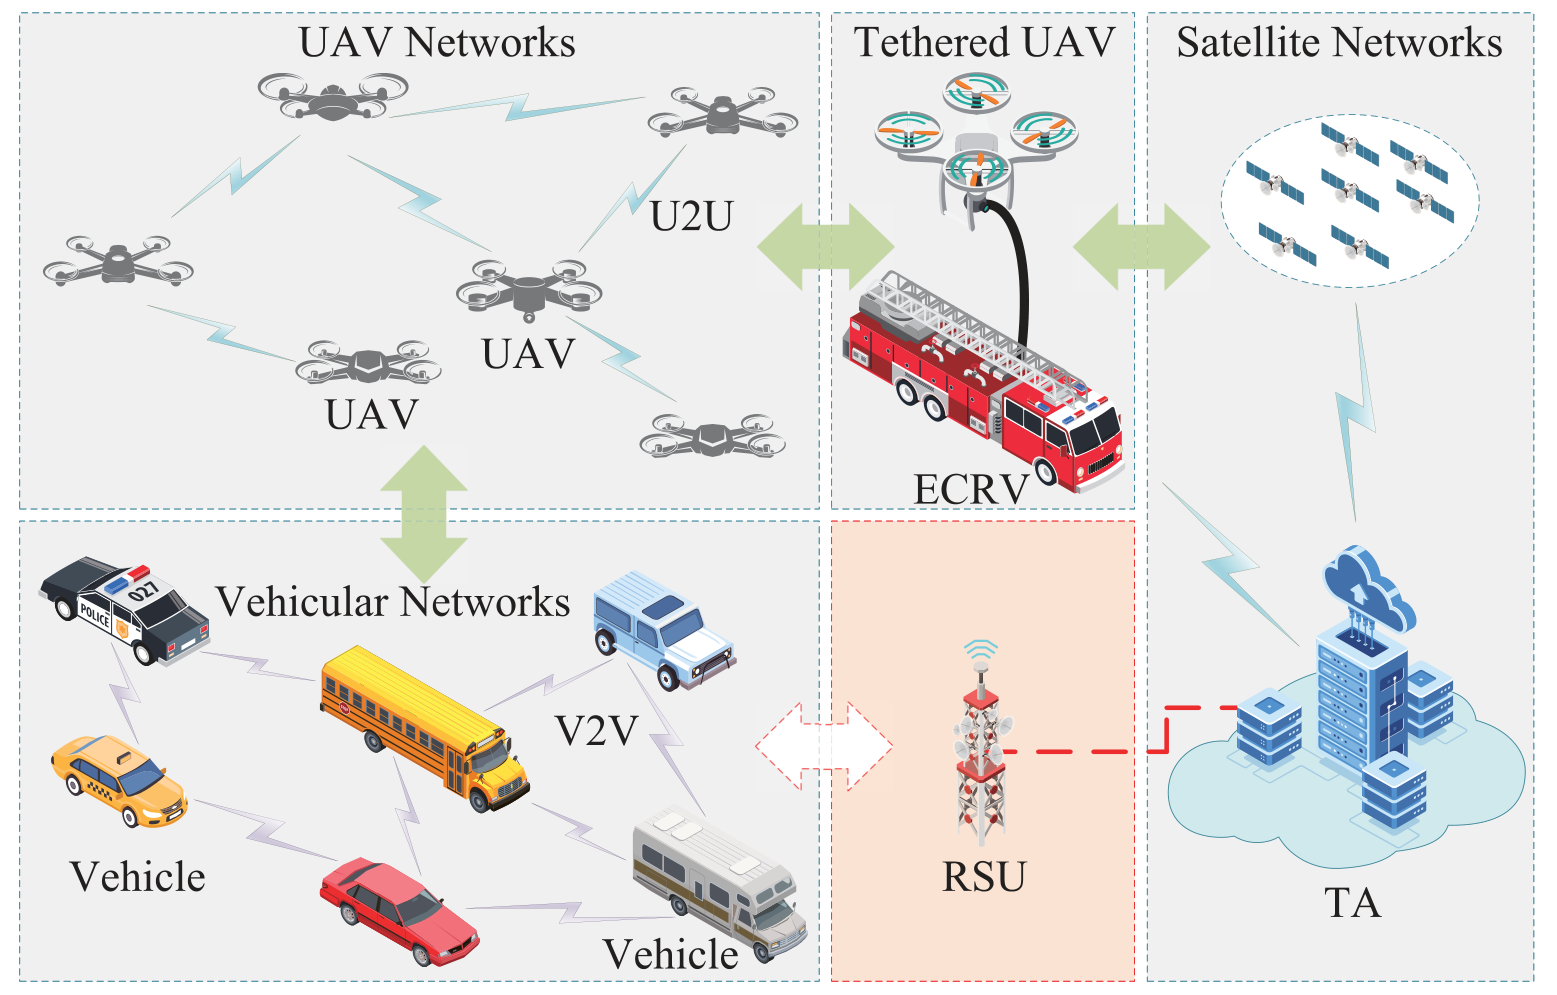
\includegraphics[width=0.78\linewidth]{paper_fig1_system_model.png}
\caption{System model of the TUAV-assisted infrastructure-less IoV, reproduced from Fig.~1 of the base paper~\cite{tan2023}. The UAV network (top left)
talks to the tethered UAV, which is powered through a cable by the ECRV. The ECRV reaches the trusted authority (TA) through the satellite network.
Vehicles (bottom left) communicate through the UAV network because the roadside unit (RSU) is out of service.}
\label{fig:sysmodel}
\end{figure}

\begin{claimbox}
``the data links between TA and TUAV are conducted with the secure communication channel, which takes the place of the dysfunctional edge RSUs.''
\quad ``the TUAVs utilize flexible tethered wires or cables as the power source instead of conventional batteries. The ECRV, as the auxiliary unit and
control center, maintains the wired power supply to the connected TUAV.'' \hfill (Section~III-D)
\end{claimbox}

\section{The protocol at a glance}
\begin{figure}[H]
\centering
\begin{tikzpicture}[font=\small,ph/.style={draw=black,fill=black!6,rounded corners=2pt,text width=11.4cm,align=left,inner sep=5pt},
  tg/.style={draw=black,fill=black!75,text=white,font=\small\bfseries,minimum width=1.9cm,minimum height=0.75cm}]
  \node[ph] (is) at (0,0) {\textbf{Initialisation} (TA, TUAV). The TA gives the TUAV $\langle id_{tu},s_{tu}\rangle$ and every UAV $\langle id_i,s_i\rangle$, and keeps a copy. The TUAV broadcasts $\langle \ts_{tu},\ID_{tu},R_{tu},Q_{tu}\rangle$.};
  \node[ph,below=0.45cm of is] (us) {\textbf{UAV signing} (each UAV). The UAV picks $r_i$, computes $\xi_i=h_1(r_i)$, $\ID_i$, $\upsilon_i$ and the credential $\Gamma_i$, and sends $\langle \ts_2,\ID_i,\xi_i,\upsilon_i,\Gamma_i\rangle$ to the TUAV.};
  \node[ph,below=0.45cm of us] (ga) {\textbf{Group authentication} (TUAV and TA, over the satellite). The TA uses $s_i$ to compute $\sigma_i,\psi_i,\mu_i,\delta_i$ (three pairings per UAV); the TUAV checks all UAVs with one product equation.};
  \node[ph,below=0.45cm of ga] (gd) {\textbf{Group key distribution} (TUAV to UAVs). The TUAV builds $\Lambda(x)=\kappa_{tu}\sum_i\omega_i\varphi_i+\prod_i(x-\sigma_i)$ and sends its coefficients; each UAV computes $\kappa_{tu}=\Lambda(\sigma_i)\bmod\sigma_i$.};
  \node[ph,below=0.45cm of gd] (du) {\textbf{Dynamic key updating} (TUAV). When UAVs join or leave, the TUAV builds a new $\Lambda^{*}(x)$ with a new key $\kappa^{*}_{tu}$; remaining members keep their $\sigma_i$.};
  \foreach \a/\b in {is/us,us/ga,ga/gd,gd/du}{\draw[-{Stealth[length=2.4mm]},thick] (\a.south) -- (\b.north);}
  \foreach \n/\t in {is/IS1--IS5,us/US1--US3,ga/GA1--GA4,gd/GD1--GD6,du/DU1--DU2}{\node[tg,left=0.25cm of \n] {\t};}
  \draw[-{Stealth[length=2.4mm]},thick,dashed] (du.east) -- ++(0.6,0) |- node[pos=0.25,right,font=\scriptsize,align=left]{on every\\ join or leave} (gd.east);
\end{tikzpicture}
\caption{The five phases of the base scheme, in order. The step labels on the left (IS, US, GA, GD, DU) are the ones used in Section~IV of the paper.
Solid arrows show the normal order; the dashed arrow shows that a key update repeats the key-distribution computation.}
\label{fig:phases}
\end{figure}

\begin{figure}[H]
\centering
\resizebox{\linewidth}{!}{%
\begin{tikzpicture}[font=\sffamily\small]
  \node[ent=uavc] (u) at (0,0) {UAV $\U_i$};
  \node[ent=hoc]  (t) at (6.6,0) {TUAV};
  \node[ent=deep] (a) at (13.2,0) {TA (via satellite)};
  \foreach \n in {u,t,a}{\draw[life] (\n.south) -- ++(0,-11.2);}
  \draw[msg=hoc] (6.6,-1.1) -- node[lbl,above]{IS5 \;$\langle \ts_{tu},\ID_{tu},R_{tu},Q_{tu}\rangle$ (broadcast)} (0,-1.1);
  \node[act=uavc,anchor=north] at (0,-1.4) {US1--US2: pick $r_i$; \;$\xi_i=h_1(r_i)$\\ $\ID_i=h_3(id_i,\ts_2,\xi_i)$, \;$\upsilon_i$, \;$\Gamma_i$};
  \draw[msg=uavc] (0,-3.0) -- node[lbl,above]{US3 \;$\langle\text{Request},\ts_2,\ID_i,\xi_i,\upsilon_i,\Gamma_i\rangle$} (6.6,-3.0);
  \draw[msg=deep,dashed] (6.6,-3.8) -- node[lbl,above]{GA1 \;upload $\langle\ts_2,\ID_i,\xi_i,\upsilon_i\rangle$ \;(satellite)} (13.2,-3.8);
  \node[act=deep,anchor=north] at (13.2,-4.1) {GA2: find $\langle id_i,s_i\rangle$; compute\\ $\sigma_i,\ \psi_i,\ \mu_i,\ \delta_i$\\ (3 pairings per UAV)};
  \draw[msg=deep,dashed] (13.2,-5.9) -- node[lbl,above]{GA2 \;$\langle\sigma_i,\psi_i,\mu_i,\delta_i\rangle$ \;(satellite)} (6.6,-5.9);
  \node[act=hoc,anchor=north] at (6.6,-6.2) {GA3--GA4: one product check\\ GD1--GD3: $\omega_i,\varphi_i,\kappa_{tu}$, \;$\Lambda(x)$, \;$S_i$};
  \draw[msg=hoc] (6.6,-8.0) -- node[lbl,above]{GD4 \;$\langle\text{ACK},\ts_3,\ID_i,S_i,\{a_k\}_{k=0}^{n}\rangle$ \;(to each UAV)} (0,-8.0);
  \node[act=uavc,anchor=north] at (0,-8.3) {GD5: check $S_i$\\ GD6: $\kappa_{tu}=\Lambda(\sigma_i)\bmod\sigma_i$};
  \node[draw=deep,fill=deep!6,rounded corners,font=\scriptsize\sffamily,text=deep,align=center] at (9.9,-10.3)
    {dashed arrows cross the satellite link; the coefficients $\{a_k\}$ travel in the clear};
\end{tikzpicture}}
\caption{Message flow of the base scheme between a UAV $\U_i$, the TUAV and the TA. Time runs from top to bottom. Solid arrows are local radio messages; dashed arrows cross the satellite link. Boxes show the local computation of each entity.}
\label{fig:baseflow}
\end{figure}

\section{Initialisation (IS)}
\begin{stepbox}{deep}{IS1--IS5 \;(Section IV-A)}
\steplabel{deep}{IS1.} TA $\to$ TUAV: $\langle id_{tu},s_{tu}\rangle$, ``safely shared only between TA and TUAV itself during the whole time''.\\
\steplabel{deep}{IS2.} TA $\to\U_i$: $\langle id_i,s_i\rangle$; ``both the TUAV and UAV identity sets are safely stored by TA''.\\
\steplabel{deep}{IS3.} Groups $\G_1,\G_2$ of prime order $q$, generator $P$, pairing $\hat e$, hashes $\BH,h_1,h_2,h_3,h_4$.\\
\steplabel{deep}{IS4.} The TUAV, ``with the effective range covering the entire region'', picks $r_{tu}$ and computes
\[ \ID_{tu}=h_2(id_{tu},r_{tu}),\qquad R_{tu}=r_{tu}\,h_2(\ts_{tu},s_{tu}),\qquad Q_{tu}=s_{tu}\,h_2(\ID_{tu},r_{tu})\,P. \]
\steplabel{deep}{IS5.} The TUAV broadcasts $\langle\ts_{tu},\ID_{tu},R_{tu},Q_{tu}\rangle$ periodically.
\end{stepbox}

\section{UAV signing (US) and group authentication (GA)}
\begin{stepbox}{uavc}{US1--US3 \;(Section IV-B1, each UAV)}
\steplabel{uavc}{US1.} Pick random $r_i$; \;$\xi_i=h_1(r_i)$; \;$\ID_i=h_3(id_i,\ts_2,\xi_i)$.\\
\steplabel{uavc}{US2.} $\upsilon_i=h_4(\ID_i,\ID_{tu},\ts_2,\xi_i)$ and
\begin{equation}\label{eq:gamma}
\Gamma_i=\big[s_i\,h_3(\ID_i,\ts_2,s_i)\,R_{tu}-h_1(s_i\xi_i)\big]P-\upsilon_i\,h_1(r_i)\,Q_{tu}.
\end{equation}
\steplabel{uavc}{US3.} Send $\langle\text{Request},\ts_2,\ID_i,\xi_i,\upsilon_i,\Gamma_i\rangle$ to the TUAV.
\end{stepbox}

\begin{stepbox}{hoc}{GA1--GA4 \;(Section IV-B2, TUAV and TA)}
\steplabel{hoc}{GA1.} TUAV checks $\ts_2$ and $\upsilon_i$ and ``uploads'' $\langle\ts_2,\ID_i,\xi_i,\upsilon_i\rangle$ ``to the remote TA''.\\
\steplabel{hoc}{GA2.} TA recovers $\langle id_i,s_i\rangle$ for $\ID_i$ and computes, for every $i$,
\begin{gather*}
\sigma_i=h_1(s_i\xi_i)P,\qquad \psi_i=\hat e(\Gamma_i+h_1(s_i\xi_i)P,\,P),\\
\mu_i=\hat e(h_3(\ID_i,\ts_2,s_i)P,\,s_iP),\qquad \delta_i=\hat e(s_{tu}P,\,\upsilon_i\xi_iP),
\end{gather*}
and forwards $\langle\sigma_i,\psi_i,\mu_i,\delta_i\rangle_{i\in[1,n]}$ to the TUAV.\\
\steplabel{hoc}{GA3.} TUAV checks
\begin{equation}\label{eq:ga3}
\prod_{i=1}^n\psi_i\Big(\prod_{i=1}^n\delta_i\Big)^{h_2(\ID_{tu},r_{tu})}\overset{?}{=}\prod_{i=1}^n\mu_i^{R_{tu}} .
\end{equation}
\steplabel{hoc}{GA4.} ``If matches, the validity of the vehicles can be proved.''
\end{stepbox}

\begin{lemma}[Correctness of GA3, the paper's Eq.~(1)]\label{lem:ga3}
For honestly generated requests, Eq.~\eqref{eq:ga3} holds.
\end{lemma}
\begin{proof}
Write $h_2=h_2(\ID_{tu},r_{tu})$ and $h_3=h_3(\ID_i,\ts_2,s_i)$. By \eqref{eq:gamma} and $h_1(r_i)=\xi_i$,
$\Gamma_i+h_1(s_i\xi_i)P=s_ih_3R_{tu}P-\upsilon_i\xi_iQ_{tu}$, so by bilinearity
$\psi_i=\hat e(s_ih_3R_{tu}P,P)\cdot\hat e(\upsilon_i\xi_iQ_{tu},P)^{-1}$. Since $Q_{tu}=s_{tu}h_2P$,
$\delta_i^{h_2}=\hat e(s_{tu}h_2P,\upsilon_i\xi_iP)=\hat e(\upsilon_i\xi_iQ_{tu},P)$. The two factors cancel and
$\psi_i\delta_i^{h_2}=\hat e(h_3P,s_iP)^{R_{tu}}=\mu_i^{R_{tu}}$. Multiply over $i$.
\end{proof}

\section{Group key distribution (GD) and dynamic update (DU)}
\begin{stepbox}{hoc}{GD1--GD6 \;(Section IV-C)}
\steplabel{hoc}{GD1.} TUAV takes the decrypting keys $\sigma_i=h_1(s_i\xi_i)P$, builds $\omega_i=\prod_{j\neq i}\sigma_j$ and $\varphi_i\equiv\omega_i^{-1}\bmod\sigma_i$,
and selects the group key $\kappa_{tu}\in\Zq$.\\
\steplabel{hoc}{GD2.} TUAV constructs
\begin{equation}\label{eq:lambda}
\Lambda(x)=\kappa_{tu}\sum_{i=1}^n\omega_i\varphi_i+\prod_{i=1}^n(x-\sigma_i)=\sum_{k=0}^{n}a_kx^k .
\end{equation}
\steplabel{hoc}{GD3.} $S_i=\BH(\ts_3,\ID_i,\,s_{tu}h_2(\ID_{tu},r_{tu})\,\sigma_i)$; the acknowledgement ``is delivered one by one to each vehicle''.\\
\steplabel{hoc}{GD4.} Packet $\langle\text{ACK},\ts_3,\ID_i,S_i,\{a_k\}_{k\in[0,n]}\rangle$.\\
\steplabel{uavc}{GD5.} UAV checks $S_i\overset{?}{=}\BH(\ts_3,\ID_i,h_1(s_i\xi_i)Q_{tu})$.\\
\steplabel{uavc}{GD6.} UAV rebuilds $\Lambda(x)$ from $\{a_k\}$ and computes $\kappa_{tu}=\Lambda(\sigma_i)\bmod\sigma_i$.
\end{stepbox}
\begin{stepbox}{hoc}{DU1--DU2 \;(Section IV-D)}
\steplabel{hoc}{DU1.} For $\ominus$ removed and $\oplus$ joining UAVs, the TUAV picks $\kappa^*_{tu}$ and computes
$\Lambda^*(x)=\prod_{i=1}^{n-\ominus+\oplus}(x-\sigma_i)+\kappa^*_{tu}\big(\sum_{i=1}^{n-\ominus+\oplus}\omega_i\varphi_i\big)$.\\
\steplabel{uavc}{DU2.} ``all the legitimate UAVs could easily extract $\kappa^*_{tu}$ with $\kappa_{tu}=\Lambda^*(\sigma_i)\bmod\sigma_i$'' -- using the
\emph{same} $\sigma_i$ as before.
\end{stepbox}

\begin{lemma}[Correctness of GD6 by the CRT]\label{lem:gd6}
If the $\sigma_i$ are pairwise coprime and $\kappa_{tu}<\sigma_i$ for all $i$, then $\Lambda(\sigma_i)\bmod\sigma_i=\kappa_{tu}$ for every member $i$.
\end{lemma}
\begin{proof}
At $x=\sigma_i$ the product in \eqref{eq:lambda} contains the factor $(\sigma_i-\sigma_i)=0$, so $\Lambda(\sigma_i)=\kappa_{tu}\sum_j\omega_j\varphi_j$.
For $j\neq i$, $\omega_j$ contains the factor $\sigma_i$, so $\omega_j\varphi_j\equiv0\pmod{\sigma_i}$; and $\omega_i\varphi_i\equiv1\pmod{\sigma_i}$ by
the choice of $\varphi_i$ (Theorem~\ref{thm:crt}). Hence $\Lambda(\sigma_i)\equiv\kappa_{tu}\pmod{\sigma_i}$, and as $\kappa_{tu}<\sigma_i$ the remainder
is $\kappa_{tu}$ itself.
\end{proof}

\begin{remark}[Point or integer?]\label{rem:typing}
The paper writes $\sigma_i=h_1(s_i\xi_i)P$, a curve point, yet uses it as a CRT modulus and as a root of a polynomial over the integers. Any
implementation must therefore map $\sigma_i$ to an integer (for instance a fixed integer encoding of the point, or a prime derived from the same hash),
and the coefficients $a_k$ must be kept as integers -- otherwise ``$\bmod\ \sigma_i$'' in GD6 is undefined. All our results hold for \emph{every} such
integer reading; nothing depends on which encoding is chosen.
\end{remark}

\section{What the paper claims}
\begin{claimbox}
\textbf{Section IV-D:} ``the group key updating mechanism supports multi-device revocation and new device participation \dots\ the dynamic key batch
updating process can be securely executed in the open wireless environment since the malicious entities that successfully collect the coefficient set
$\{a_i\}_{i\in[0,n]}$ can not acquire the $\kappa_{tu}$ without the correct decrypting key $\sigma_i$.''\\[3pt]
\textbf{Proof of Theorem 4:} ``The certificateless authentication is adopted, where the partial secret set $\langle s_i,s_{tu}\rangle$ of TUAV and UAVs is
generated and determined by TA. On the other hand, the UAV itself also randomly generates $r_i$ as the partial key \dots''\\[3pt]
\textbf{Proof of Theorem 5:} ``The remaining legitimate UAVs could always use the previously issued key to decrypt the new $\kappa_{tu}$ with the updated
$\Lambda(x)$, if the $\sigma_i$ has not been removed by TUAV.''\\[3pt]
\textbf{Table II:} the proposed scheme is ticked (\yes) for all of F1--F11: unforgeability, conditional privacy, session key establishment,
\textbf{key escrow resilience}, scalability, dynamic identity updating, \textbf{forward secrecy}, batch validation, unlinkability,
\textbf{non-repudiation} and replay attack resilience.
\end{claimbox}

\begin{center}
\small
\begin{tabularx}{\linewidth}{@{}X c X@{}}
\toprule
\textbf{Claim in~\cite{tan2023}} & \textbf{Paper} & \textbf{This report}\\
\midrule
Key escrow resilience (Table II, F4) & \yes & \no\ fails: the TA can sign for any UAV (F1, Theorem~\ref{thm:taforge})\\
Non-repudiation (Table II, F10) & \yes & \no\ fails: the TA could have produced any request (F1)\\
``supports multi-device revocation'' (IV-D, Thm.~5) & \yes & \no\ fails: a removed UAV computes the new key (F2a)\\
New-device participation is secure (IV-D) & \yes & \no\ fails: a newcomer reads old keys (F2b)\\
Coefficients reveal nothing without a $\sigma_i$ (IV-D) & \yes & \no\ fails: a passive outsider gets all keys (F2c)\\
Forward secrecy (Table II, F7) & \yes & \no\ fails: a leaked $s_i$ opens all past keys (F3)\\
\bottomrule
\end{tabularx}
\end{center}

% =====================================================================
\chapter{Security and performance analysis in the paper}\label{ch:p1analysis}
% =====================================================================
\section{Security analysis in the paper}
Section~V of the paper gives five theorems. We summarise each one and how the paper argues it.
\begin{center}
\small
\begin{tabularx}{\linewidth}{@{}p{3.8cm} X@{}}
\toprule
\textbf{Theorem (paper)} & \textbf{What it claims and how it is argued}\\
\midrule
1 -- Message unforgeability & secure against chosen-message attacks in the random-oracle model if CDH is hard; the proof embeds the CDH instance
$(s_{tu}P,\ (\sum_i\upsilon_i\xi_i)P)$ and uses two forgeries with different $h_2$ values\\
2 -- User anonymity and unlinkability & temporary identities $\ID_i=h_3(id_i,\ts_2,\xi_i)$ change every session, so eavesdroppers cannot link messages\\
3 -- Replay attack resistance & every credential includes a fresh timestamp, so old messages fail the current check\\
4 -- Conditional privacy & real identities stay hidden, but the law-enforcement agency can reveal a malicious UAV when the TA reports it\\
5 -- Session key establishment & every verified UAV gets the same group key $\kappa_{tu}=\Lambda(\sigma_i)\bmod\sigma_i$; remaining UAVs can decrypt
updated keys ``if the $\sigma_i$ has not been removed by TUAV''\\
\bottomrule
\end{tabularx}
\end{center}
In its Table~II the paper compares itself with four earlier schemes on eleven properties (F1--F11) and ticks all eleven for itself, including
\emph{key escrow resilience}, \emph{forward secrecy} and \emph{non-repudiation}.

\section{Performance analysis in the paper}
The paper measures basic operations with the MIRACL library at an 80-bit security level: a supersingular curve with a 512-bit field for the pairing
group $\G_1$, and an ordinary 160-bit curve for the group $\G$.
\begin{center}
\small
\begin{tabular}{@{}l l r@{}}
\toprule
\textbf{Symbol} & \textbf{Operation} & \textbf{Time (ms)}\\
\midrule
$T_P$ & bilinear pairing & 7.2232\\
$T_{SM\cdot P}$ & scalar multiplication in $\G_1$ & 2.6784\\
$T_{H\cdot MP\cdot P}$ & MapToPoint hash & 8.1940\\
$T_{SM\cdot E}$ & scalar multiplication on the ordinary curve & 0.9018\\
$T_{PA\cdot E}$ & point addition on the ordinary curve & 0.0107\\
$T_{ME}$ & modular exponentiation & 0.6256\\
$T_{SH}$ & hash & 0.0012\\
\bottomrule
\end{tabular}
\end{center}
With these constants the paper reports: UAV signing (US) $2T_{SM\cdot E}+T_{PA\cdot E}+5T_{SH}\approx1.82$\,ms, single verification (SA)
$\approx2.16$\,ms, and group authentication (GA) $1.2524n+0.9054$\,ms, i.e.\ about $151$\,ms for $n=120$ UAVs. For GA the paper notes that the pairing
work is done by the TA ``prior to the verification of TUAV'', so it counts the TUAV side.

\begin{figure}[H]
\centering
\begin{tikzpicture}
\begin{axis}[width=0.88\linewidth,height=6.6cm,xmin=0,xmax=120,ymin=0,ymax=2100,xlabel={Number of UAVs $n$},ylabel={Group-authentication time (ms)},
  xtick={0,20,...,120},grid=major,grid style={black!10},legend cell align=left,legend style={font=\footnotesize,at={(0.02,0.98)},anchor=north west,draw=black!40},
  tick label style={font=\small},label style={font=\small},mark repeat=2,scaled y ticks=false,y tick label style={/pgf/number format/.cd,fixed,1000 sep={}}]
  \addplot[thick,color=plotB,mark=square*,mark size=1.6pt,domain=0:120,samples=13] {16.2292*x+37.0868}; \addlegendentry{Kumar et al.: $16.23n+37.09$}
  \addplot[thick,color=plotD,mark=triangle*,mark size=2pt,domain=0:120,samples=13] {13.6534*x+29.7952}; \addlegendentry{Xu et al.: $13.65n+29.80$}
  \addplot[thick,color=plotC,mark=diamond*,mark size=2pt,domain=0:120,samples=13] {5.4252*x+45.2124}; \addlegendentry{Mei et al.: $5.43n+45.21$}
  \addplot[thick,color=plotE,mark=o,mark size=1.6pt,domain=0:120,samples=13] {2.7126*x+7.2232}; \addlegendentry{Ali et al.: $2.71n+7.22$}
  \addplot[very thick,color=plotA,mark=*,mark size=1.6pt,domain=0:120,samples=13] {1.2524*x+0.9054}; \addlegendentry{Base paper (TUAV side): $1.25n+0.91$}
  \node[font=\footnotesize,anchor=south east] at (axis cs:119,165) {151 ms at $n=120$};
\end{axis}
\end{tikzpicture}
\caption{Group-authentication (GA) time against the number of UAVs, plotted from the cost formulas in Section~VI-A of the base paper for the four schemes
it compares with (Kumar et al., Xu et al., Mei et al., Ali et al.) and for itself. The base paper's line counts only the TUAV side; the TA's pairings
are not included.}
\label{fig:p1cost}
\end{figure}

For communication, the paper uses 128-byte elements in $\G_1$, 40-byte elements in $\G$, 20-byte hashes and 4-byte timestamps, and reports lower
overhead than the four compared schemes (its Table~V).

\section{Open questions we took forward}
While studying the paper we noted several points that we wanted to check carefully:
\begin{enumerate}[leftmargin=*]
\item The TA stores every UAV's secret $s_i$ (IS2), yet the paper claims key-escrow resilience and non-repudiation. \hfill $\rightarrow$ F1
\item The coefficients of $\Lambda(x)$ are sent in the clear and only the constant term is masked. \hfill $\rightarrow$ F2
\item The decrypting key $\sigma_i=h_1(s_i\xi_i)P$ uses no fresh secret, yet forward secrecy is claimed. \hfill $\rightarrow$ F3
\item Every login goes through the TA over the satellite, and only one TUAV is assumed for the whole region (IS4). \hfill $\rightarrow$ C1, C2
\item Nothing is said about a TUAV that is hacked or physically captured. \hfill $\rightarrow$ C3, C4
\end{enumerate}


% ============================== analysis and contributions ==============================

% =====================================================================
\chapter{Our analysis and contributions: overview}\label{ch:p2overview}
% =====================================================================
\section{Our approach}
We treated the paper's printed equations as the source of truth. For every security claim we asked: \emph{what exactly does an attacker
know, and what can it compute from that?} When a claim failed, we wrote the failure as a theorem with a proof and a small example that can be checked
by hand. We then read related literature (CRT and polynomial group keys, certificateless signatures, batch verification, mediated and threshold
signatures, Byzantine fault tolerance) and designed fixes that use well-known tools in a new place.

\section{Results at a glance}
\begin{center}
\small
\begin{tabularx}{\linewidth}{@{}l X l@{}}
\toprule
& \textbf{Result} & \textbf{Chapter}\\
\midrule
\textcolor{bad}{\textbf{F1}} & \textbf{TA impersonation:} the TA can produce a valid request for any UAV; key-escrow resilience and non-repudiation fail. & \ref{ch:f1}\\
\textcolor{bad}{\textbf{F2}} & \textbf{CRT group-key leakage:} a removed UAV reads new keys, a newcomer reads old keys, and a passive outsider who records two
broadcasts recovers every key. & \ref{ch:f2}\\
\textcolor{bad}{\textbf{F3}} & \textbf{No forward secrecy:} one leaked long-term secret opens all past group keys. & \ref{ch:f3}\\
\midrule
\textcolor{uavc}{\textbf{C1}} & \textbf{Authentication with the TA offline} and a separately sealed key for every member. & \ref{ch:c1}\\
\textcolor{hoc}{\textbf{C2}} & \textbf{Handover between TUAVs} with a one-time ticket and signatures in both directions. & \ref{ch:c2}\\
\textcolor{quorum}{\textbf{C3}} & \textbf{Quorum eviction:} $t$ TUAVs vote out a compromised TUAV. & \ref{ch:c3}\\
\textcolor{tether}{\textbf{C4}} & \textbf{Tether-split key:} a captured drone holds only half a key and cannot sign. & \ref{ch:c4}\\
\textbf{A1--A7} & \textbf{Hardening:} seven flaws we found in our own first design and fixed. & \ref{ch:hard}\\
\bottomrule
\end{tabularx}
\end{center}

\begin{figure}[H]
\centering
\resizebox{\linewidth}{!}{%
\begin{tikzpicture}[font=\sffamily\small,b/.style={draw=black,rounded corners=3pt,align=center,inner sep=5pt,text width=#1},
  ar/.style={-{Stealth[length=3mm]},very thick}]
  \node[font=\sffamily\bfseries] at (0,3.9) {Weaknesses found};
  \node[font=\sffamily\bfseries] at (7.2,3.9) {Fix};
  \node[font=\sffamily\bfseries] at (14.6,3.9) {Gaps that remain};
  \node[font=\sffamily\bfseries] at (20.4,3.9) {Further contributions};
  \node[b=4.2cm,fill=black!12] (f1) at (0,2.4) {\textbf{F1} TA impersonation\\ \scriptsize key escrow, no non-repudiation};
  \node[b=4.2cm,fill=black!12] (f2) at (0,0) {\textbf{F2} CRT key leakage\\ \scriptsize insider and passive outsider};
  \node[b=4.2cm,fill=black!12] (f3) at (0,-2.4) {\textbf{F3} no forward secrecy\\ \scriptsize one leak opens the past};
  \node[b=4.4cm,fill=white,minimum height=2.8cm,line width=1.2pt] (c1) at (7.2,0) {\textbf{C1}\\ TA-offline certificateless authentication and per-member key delivery};
  \foreach \f in {f1,f2,f3}{\draw[ar] (\f.east) -- (c1.west);}
  \node[b=4.3cm,fill=black!5] (g1) at (14.6,2.4) {\scriptsize only one TUAV ``covering the entire region'' (IS4)};
  \node[b=4.3cm,fill=black!5] (g2) at (14.6,0) {\scriptsize no way to remove a compromised TUAV while the TA is offline};
  \node[b=4.3cm,fill=black!5] (g3) at (14.6,-2.4) {\scriptsize a captured TUAV keeps its whole key};
  \node[b=3.4cm,fill=white,line width=1.2pt] (c2) at (20.4,2.4) {\textbf{C2} handover};
  \node[b=3.4cm,fill=white,line width=1.2pt] (c3) at (20.4,0) {\textbf{C3} quorum eviction};
  \node[b=3.4cm,fill=white,line width=1.2pt] (c4) at (20.4,-2.4) {\textbf{C4} tether-split key};
  \draw[ar] (g1.east) -- (c2.west); \draw[ar] (g2.east) -- (c3.west); \draw[ar] (g3.east) -- (c4.west);
  \draw[ar,dashed] (c1.east) -- node[above,font=\scriptsize\sffamily,align=center]{after C1 the TUAV\\ holds the trust} (g2.west);
  \node[b=22.6cm,fill=black!5] at (10.2,-4.3) {\textbf{A1--A7}: seven flaws found in our own first design and fixed (one found only by formal verification)};
\end{tikzpicture}}
\caption{How our results fit together. Left: the three weaknesses we prove in the base scheme. They are all removed by contribution C1. After C1 the TA is
offline, so the TUAV becomes the trusted party; this leaves three gaps (third column), which are closed by C2, C3 and C4. A1--A7 are improvements to
our own design.}
\label{fig:map}
\end{figure}

% =====================================================================
\chapter{F1: the TA can impersonate any UAV}\label{ch:f1}
% =====================================================================
\begin{flawbox}[title={Flaw F1 -- key escrow: the TA can sign as any UAV}]
The TA stores every UAV's long-term secret $s_i$ (IS2), and every other input of the credential $\Gamma_i$ is public. Hence the TA -- or anyone who
steals the TA's database -- can produce a request that GA1--GA4 accept in the name of \emph{any} UAV, and nobody can tell it from a genuine one. Two
properties ticked in the paper's Table~II fail: \textbf{key-escrow resilience} and \textbf{non-repudiation}.
\end{flawbox}

\section{Who knows what}
Look at the credential of Eq.~\eqref{eq:gamma}, $\Gamma_i=\big[s_i\,h_3(\ID_i,\ts_2,s_i)\,R_{tu}-h_1(s_i\xi_i)\big]P-\upsilon_i\,h_1(r_i)\,Q_{tu}$:
\begin{center}
\begin{tabular}{@{}l c c c l@{}}
\toprule
\textbf{Input of $\Gamma_i$} & \textbf{UAV} & \textbf{TA} & \textbf{Everyone} & \textbf{Source}\\
\midrule
$s_i$ (long-term secret) & \yes & \yes & \no & IS2: issued and stored by the TA\\
$r_i$ (random) & \yes & \no & \no & US1\\
$h_1(r_i)=\xi_i$ & \yes & \yes & \yes & sent in the clear in US3\\
$\ID_i,\ \upsilon_i,\ \ts_2$ & \yes & \yes & \yes & sent in the clear in US3\\
$R_{tu},\ Q_{tu},\ \ID_{tu}$ & \yes & \yes & \yes & TUAV beacon, IS5\\
\bottomrule
\end{tabular}
\end{center}
The only value outside the TA's reach is $r_i$, and $r_i$ enters $\Gamma_i$ \emph{only} through $h_1(r_i)=\xi_i$, which is public.

\section{The theorem}
\begin{theorem}[TA forgery]\label{thm:taforge}
Any party that knows $\langle id_i,s_i\rangle$ can, in polynomial time and without any value chosen by UAV $i$, produce a request that passes GA1--GA4
in the name of UAV $i$, and then obtain the group key through GD4--GD6.
\end{theorem}
\begin{proof}
The forger runs Algorithm~\ref{alg:forge}. Its output has exactly the form of an honest request in which the public value $\xi'$ plays the role of
$h_1(r_i)$. The correctness argument of Lemma~\ref{lem:ga3} uses only the identity $h_1(r_i)=\xi_i$ and the definitions of $\upsilon_i$, $R_{tu}$ and
$Q_{tu}$ -- never the value $r_i$ itself -- so it applies verbatim with $(\xi',\ts',\ID',\upsilon',\Gamma')$, and GA3 holds. In GD5 the forger computes
$\BH(\ts_3,\ID',h_1(s_i\xi')Q_{tu})$ from known values, and in GD6 it computes $\sigma'=h_1(s_i\xi')P$ and $\kappa_{tu}=\Lambda(\sigma')\bmod\sigma'$.
Every step costs a constant number of hash evaluations and scalar multiplications.
\end{proof}

\begin{algorithm}{Forge$(id_i,s_i)$ -- impersonate UAV $i$}\label{alg:forge}
\begin{enumerate}[leftmargin=*,label=\arabic*.]
\item Read the current beacon $\langle\ts_{tu},\ID_{tu},R_{tu},Q_{tu}\rangle$ (IS5).
\item Pick any $\xi'\in\Zq$ and a fresh timestamp $\ts'$ -- no $r'$ is ever needed.
\item $\ID'=h_3(id_i,\ts',\xi')$, \quad $\upsilon'=h_4(\ID',\ID_{tu},\ts',\xi')$.
\item $\Gamma'=\big[s_i\,h_3(\ID',\ts',s_i)\,R_{tu}-h_1(s_i\xi')\big]P-\upsilon'\,\xi'\,Q_{tu}$.
\item Send $\langle\text{Request},\ts',\ID',\xi',\upsilon',\Gamma'\rangle$ to the TUAV. GA1--GA4 accept.
\item On $\langle\text{ACK},\ts_3,\ID',S',\{a_k\}\rangle$: $\sigma'=h_1(s_i\xi')P$, \;$\kappa_{tu}=\Lambda(\sigma')\bmod\sigma'$.
\end{enumerate}
\end{algorithm}

\begin{figure}[H]
\centering
\resizebox{\linewidth}{!}{%
\begin{tikzpicture}[font=\sffamily\small,node distance=0.5cm]
  \node[fstart=bad] (s) {TA database\\ $\langle id_i,s_i\rangle$ (stored in IS2)};
  \node[fproc=bad,right=of s,text width=3.0cm] (a) {pick public $\xi'$ and fresh $\ts'$;\\ $\ID',\ \upsilon'$};
  \node[fproc=bad,right=of a,text width=3.4cm] (b) {$\Gamma'$ from Eq.~\eqref{eq:gamma} with\\ $h_1(r_i)$ replaced by $\xi'$};
  \node[fproc=deep,right=of b,text width=3.1cm] (c) {TUAV and TA run\\ GA1--GA4 honestly};
  \node[fdec=deep,right=of c] (d) {GA3\\ holds?};
  \node[fstart=bad,below=1.0cm of d,text width=3.4cm] (e) {\textbf{accepted as UAV $i$}\\ + group key $\kappa_{tu}$ via GD6};
  \draw[flow] (s) -- (a); \draw[flow] (a) -- (b); \draw[flow] (b) -- (c); \draw[flow] (c) -- (d);
  \draw[flow] (d) -- node[lbl,right]{always yes (Lemma~\ref{lem:ga3})} (e);
\end{tikzpicture}}
\caption{Flowchart of the TA-forgery attack (Algorithm~\ref{alg:forge}). Starting from the stored pair $\langle id_i,s_i\rangle$, the forger builds a request with a public $\xi'$; the honest TUAV and TA then accept it. No step uses a value chosen by the real UAV.}
\label{fig:f1flow}
\end{figure}

\section{Consequences}
\begin{corollary}[Key escrow and repudiation]\label{cor:escrow}
(i) The base scheme is at Girault trust level~1: the authority can impersonate any user without leaving a trace. Key-escrow resilience (Table~II,
F4) does not hold. (ii) Non-repudiation (Table~II, F10) does not hold: for any accepted request, the TA could have produced it. Moreover, only the TA
can verify a request at all, since $\mu_i=\hat e(h_3(\ID_i,\ts_2,s_i)P,\,s_iP)$ needs $s_i$; a third party can never check a UAV's message.
\end{corollary}

\begin{corollary}[The TA reads every group key]
In GA2 the TA computes every $\sigma_i$, so it can evaluate $\kappa_{tu}=\Lambda(\sigma_i)\bmod\sigma_i$ for every broadcast it observes.
\end{corollary}

\begin{remark}[The ``certificateless'' claim]
The proof of Theorem~4 states that ``the certificateless authentication is adopted'' with ``$r_i$ as the partial key''. In a certificateless scheme the
user's own secret must enter the \emph{signing key}, so that the authority's partial key alone is useless~\cite{alriyami}. Here $r_i$ enters only as
$h_1(r_i)=\xi_i$, and $\xi_i$ is broadcast in US3. The user's ``partial key'' therefore contributes no secret, and the scheme is, in effect, a
key-escrow scheme.
\end{remark}

\begin{remark}[Why the paper's Theorem~1 does not catch this]
The reduction of Theorem~1 lets an adversary $\mathcal A_1$ forge requests, but $\mathcal A_1$ is never given what the TA knows. A malicious or
breached authority (a ``Type~II'' adversary in certificateless terminology~\cite{alriyami}) is outside the model, which is exactly the case of F1.
\end{remark}


\begin{fixbox}[title={How C1 removes F1 (Chapter~\ref*{ch:c1})}]
Each UAV adds its own secret $x$ that never leaves the device: $\sk=x+d$. The TA knows only the partial key $d$, so it cannot sign under the UAV's
key (Theorem~\ref{thm:noescrow}).
\end{fixbox}

% =====================================================================
\chapter{F2: the CRT group key leaks -- to members and to outsiders}\label{ch:f2}
% =====================================================================
\begin{flawbox}[title={Flaw F2 -- the broadcast polynomial reveals the decrypting keys}]
The polynomial $\Lambda(x)=\kappa_{tu}\sum_i\omega_i\varphi_i+\prod_i(x-\sigma_i)$ hides only its \emph{constant} term. Every other coefficient is a
symmetric function of the members' decrypting keys, published in the clear.
\begin{itemize}[leftmargin=*]
\item \textbf{F2(a) -- revocation fails.} Any member recovers \emph{every} $\sigma_i$; after being removed it still computes each new group key.
\item \textbf{F2(b) -- backward secrecy fails.} A UAV that joins recovers the old members' $\sigma_i$ and opens recorded old group keys.
\item \textbf{F2(c) -- a passive outsider wins.} An eavesdropper who never registered records the two broadcasts around one join or leave and recovers
every $\sigma_i$ and \emph{both} group keys.
\end{itemize}
\end{flawbox}

\section{One value is the same for everybody}
\begin{lemma}[Common value]\label{lem:common}
Let $C=\kappa_{tu}\sum_{i=1}^n\omega_i\varphi_i$. Then $\Lambda(\sigma_j)=C$ for every member $j$.
\end{lemma}
\begin{proof}
At $x=\sigma_j$ the product $\prod_i(x-\sigma_i)$ contains the factor $(\sigma_j-\sigma_j)=0$, so only the constant $C$ remains.
\end{proof}
\noindent The paper uses this fact to deliver the key ($C\bmod\sigma_j=\kappa_{tu}$, Lemma~\ref{lem:gd6}). But the same fact means that every member
knows the \emph{mask} $C$ itself, not only $C\bmod\sigma_j$.

\section{The insider attack: F2(a) and F2(b)}
\begin{theorem}[Insider key recovery]\label{thm:insider}
A member $j$ that knows only its own $\sigma_j$ and the broadcast coefficients $\{a_k\}$ recovers every member's decrypting key in polynomial time.
\end{theorem}
\begin{proof}
By Lemma~\ref{lem:common} member $j$ computes $C=\Lambda(\sigma_j)$, so it knows
\[
\boxed{\;\Lambda(x)-C=\prod_{i=1}^{n}(x-\sigma_i)\;}
\]
-- the broadcast polynomial with $a_0$ replaced by $a_0-C$. This is a monic integer polynomial whose roots are exactly the $\sigma_i$; all of them are
integers (Remark~\ref{rem:typing}), so by the Rational Root Theorem (\ref{thm:rrt}) and Proposition~\ref{prop:roots} they are found in time polynomial in
$n$ and the bit length.
\end{proof}

\begin{corollary}[F2(a): revocation fails]\label{cor:revoke}
Let member $j$ be removed by DU1 and let $k$ be any member that stays. From the broadcast before its removal, $j$ knows $\sigma_k$
(Theorem~\ref{thm:insider}); DU2 keeps $\sigma_k$ unchanged; hence $j$ computes the new key $\kappa^*_{tu}=\Lambda^*(\sigma_k)\bmod\sigma_k$.
\end{corollary}

\begin{corollary}[F2(b): backward secrecy fails]\label{cor:backward}
Let UAV $k$ join in DU1. Applying Theorem~\ref{thm:insider} to $\Lambda^*$, it learns the decrypting keys of the old members, which DU2 kept unchanged. For
any recorded earlier broadcast $\Lambda$ and any old member $j$, it computes the old key $\kappa_{tu}=\Lambda(\sigma_j)\bmod\sigma_j$.
\end{corollary}

\begin{figure}[H]
\centering
\resizebox{\linewidth}{!}{%
\begin{tikzpicture}[font=\sffamily\small,node distance=0.45cm]
  \node[fio=bad,text width=2.5cm] (in) {receive $\{a_k\}$ (GD4) as a member $j$};
  \node[fproc=bad,right=of in,text width=2.4cm] (c) {$C=\Lambda(\sigma_j)$\\ (Lemma~\ref{lem:common})};
  \node[fproc=bad,right=of c,text width=2.7cm] (p) {$\Lambda(x)-C=\prod_i(x-\sigma_i)$};
  \node[fproc=vehc,right=of p,text width=2.5cm] (r) {integer roots\\ (Prop.~\ref{prop:roots})\\ $\Rightarrow$ all $\sigma_i$};
  \node[fdec=bad,right=of r] (d) {later\\ event?};
  \node[fstart=bad,above right=0.2cm and 0.7cm of d,text width=3.4cm] (a) {\textbf{F2(a)} removed: $\kappa^*=\Lambda^*(\sigma_k)\bmod\sigma_k$};
  \node[fstart=bad,below right=0.2cm and 0.7cm of d,text width=3.4cm] (b) {\textbf{F2(b)} joined: old $\kappa=\Lambda(\sigma_j)\bmod\sigma_j$};
  \draw[flow] (in) -- (c); \draw[flow] (c) -- (p); \draw[flow] (p) -- (r); \draw[flow] (r) -- (d);
  \draw[flow] (d) |- node[lbl,pos=0.3,left]{revoked} (a); \draw[flow] (d) |- node[lbl,pos=0.3,left]{newcomer} (b);
\end{tikzpicture}}
\caption{Flowchart of the insider attack (Theorem~\ref{thm:insider}). A member evaluates the broadcast polynomial at its own key, subtracts the result and finds the roots; this gives every member's key. Depending on what happens later, the same member can break revocation, F2(a), or backward secrecy, F2(b).}
\label{fig:insiderflow}
\end{figure}



\section{The passive outsider attack: F2(c)}
The insider attack needs one $\sigma_j$. The outsider attack needs none: it uses only the public coefficients of two broadcasts.

\begin{lemma}[Vieta sum leak]\label{lem:sum}
If $n\ge2$, the coefficient $a_{n-1}$ of $\Lambda(x)$ equals $-(\sigma_1+\dots+\sigma_n)$. More generally $a_k$ for $1\le k\le n-1$ are the coefficients of
$\prod_i(x-\sigma_i)$ exactly, without any mask.
\end{lemma}
\begin{proof}
The mask $C$ is a constant, so it changes only $a_0$. The remaining coefficients are those of $\prod_i(x-\sigma_i)$, given by Vieta's formulas
(Theorem~\ref{thm:vieta}); in particular $a_{n-1}=-e_1(\sigma)=-\sum_i\sigma_i$.
\end{proof}

\begin{theorem}[Passive outsider key recovery]\label{thm:outsider}
Let $\Lambda$ and $\Lambda'$ be two consecutive broadcasts whose member sets differ by exactly one UAV with key $\sigma$, and suppose at least two members
are common to both sets. An eavesdropper that knows only $\{a_k\}$ and $\{a'_k\}$ computes, in polynomial time, $\sigma$, every other decrypting key, the
old group key $\kappa_{tu}$ and the new group key $\kappa^*_{tu}$.
\end{theorem}
\begin{proof}
Write $p(x)=\prod_{\text{old}}(x-\sigma_i)=\sum p_kx^k$ and $q(x)=\prod_{\text{new}}(x-\sigma_i)=\sum q_kx^k$. By Lemma~\ref{lem:sum} the eavesdropper
knows every coefficient of $p$ and $q$ except the constants $p_0$ and $q_0$.

\emph{Leave} ($\deg q=\deg p-1$). Then $p(x)=(x-\sigma)\,q(x)$. The sums are public, so $\sigma=-p_{n-1}+q_{n-2}$. Comparing the coefficients of $x^1$
in $p=(x-\sigma)q$ gives $p_1=q_0-\sigma q_1$, hence
\[
\boxed{\;q_0=p_1+\sigma\,q_1\;}
\]
where $p_1=a_1$ and $q_1=a'_1$ are public (because at least two members remain, $q_1$ is not the masked constant). Now $q$ is known completely, its roots
are the remaining keys (Proposition~\ref{prop:roots}), and $p=(x-\sigma)q$ is known too. With any key, the attacker evaluates $\Lambda(\sigma_j)\bmod\sigma_j$
and $\Lambda'(\sigma_j)\bmod\sigma_j$ like a member and obtains both group keys.

\emph{Join} ($\deg q=\deg p+1$). Now $q(x)=(x-\sigma)\,p(x)$, $\sigma=-q_{n}+p_{n-1}$, and the $x^1$ coefficients give
$\boxed{\,p_0=q_1+\sigma\,p_1\,}$; the rest is identical with the roles of $p$ and $q$ swapped.
\end{proof}

\begin{algorithm}{OutsiderRecover$(\{a_k\},\{a'_k\})$ -- two recorded broadcasts}\label{alg:outsider}
\begin{enumerate}[leftmargin=*,label=\arabic*.]
\item $n\leftarrow\deg\Lambda$, \;$n'\leftarrow\deg\Lambda'$. If $|n-n'|\neq1$, stop (outside the theorem).
\item Sums: $S=-a_{n-1}$, \;$S'=-a'_{n'-1}$; \;$\sigma\leftarrow|S-S'|$.
\item If $n'=n-1$ (leave): $q_0\leftarrow a_1+\sigma\,a'_1$; \;$f(x)\leftarrow x^{n'}+a'_{n'-1}x^{n'-1}+\dots+a'_1x+q_0$ (the new product).\\
If $n'=n+1$ (join): $p_0\leftarrow a'_1+\sigma\,a_1$; \;$f(x)\leftarrow x^{n}+a_{n-1}x^{n-1}+\dots+a_1x+p_0$ (the old product).
\item Find the integer roots of $f$ (Proposition~\ref{prop:roots}); together with $\sigma$ these are all keys of both sets.
\item Output $\kappa_{tu}=\Lambda(\sigma_j)\bmod\sigma_j$ and $\kappa^*_{tu}=\Lambda'(\sigma_k)\bmod\sigma_k$ for any old $j$ and new $k$.
\end{enumerate}
\end{algorithm}

\begin{figure}[H]
\centering
\resizebox{\linewidth}{!}{%
\begin{tikzpicture}[font=\sffamily\small]
  \node[fio=deep,text width=2.4cm] (b0) at (0,1.1) {record broadcast\\ $\{a_k\}$ (before)};
  \node[fio=deep,text width=2.4cm] (b1) at (0,-1.1) {record broadcast\\ $\{a'_k\}$ (after)};
  \node[fproc=bad,text width=2.9cm] (s) at (4.4,0) {sums $S=-a_{n-1}$,\\ $S'=-a'_{n'-1}$;\\ $\sigma=|S-S'|$};
  \node[fdec=bad] (d) at (8.0,0) {leave or\\ join?};
  \node[fproc=bad,text width=2.6cm] (l) at (11.6,1.3) {leave: $q_0=a_1+\sigma a'_1$};
  \node[fproc=bad,text width=2.6cm] (j) at (11.6,-1.3) {join: $p_0=a'_1+\sigma a_1$};
  \node[fproc=vehc,text width=2.6cm] (r) at (15.2,0) {full product\\ $\Rightarrow$ integer roots\\ $\Rightarrow$ all $\sigma_i$};
  \node[fstart=bad,text width=2.4cm] (o) at (18.6,0) {\textbf{old and new}\\ group keys};
  \draw[flow] (b0.east) -- (s.west); \draw[flow] (b1.east) -- (s.west); \draw[flow] (s) -- (d);
  \draw[flow] (d.north) |- node[lbl,pos=0.3,left]{$n'=n-1$} (l.west); \draw[flow] (d.south) |- node[lbl,pos=0.3,left]{$n'=n+1$} (j.west);
  \draw[flow] (l.east) -| (r.north); \draw[flow] (j.east) -| (r.south); \draw[flow] (r) -- (o);
\end{tikzpicture}}
\caption{Flowchart of the passive outsider attack (Algorithm~\ref{alg:outsider}). The attacker records the coefficient sets before and after one membership change, obtains the changed member's key from the two coefficient sums, removes the mask, and finds all keys and both group keys. It needs no registration and no secret.}
\label{fig:outflow}
\end{figure}


\subsection*{Several UAVs leaving (or joining) at once}
DU1 is a \emph{batch} update: $\ominus$ UAVs may leave or $\oplus$ may join in one step. The same algebra extends.

\begin{proposition}[Batch changes]\label{prop:batch}
Suppose $m\ge1$ UAVs leave in one update and $r\ge m+1$ members remain (or $m$ UAVs join a group of $r\ge m+1$). Then the two broadcasts determine all
keys of both groups in polynomial time.
\end{proposition}
\begin{proof}
For a leave write $p=q\cdot d$ with $q=\prod_{\text{stay}}(x-\sigma_i)$ of degree $r$ and $d=\prod_{\text{leave}}(x-\sigma_i)=x^m+d_{m-1}x^{m-1}+\dots+d_0$.
Comparing the coefficients of $x^{n-j}$ for $j=1,\dots,m$ (with $n=r+m$) gives
\[
d_{m-j}=p_{n-j}-\sum_{i=1}^{j}q_{r-i}\,d_{m-j+i},
\]
which uses only $p_{n-j}$ ($n-j\ge r\ge1$, unmasked), $q_{r-i}$ with $r-i\ge r-m\ge1$ (unmasked) and already computed $d$'s. So $d$ is found top-down.
The coefficient of $x^m$ then gives $q_0=p_m-\sum_{i=1}^{\min(m,r)}q_i\,d_{m-i}$. Now $d$ and $q$ are known; their roots are all keys. A batch join is the
same with the roles of the two broadcasts swapped.
\end{proof}


\begin{remark}[Scope]
Theorem~\ref{thm:outsider} is proved for one join or one leave between two broadcasts, and Proposition~\ref{prop:batch} for batches of pure leaves or pure
joins with more members staying than changing. Two cases remain open: a \emph{single} broadcast with no
second one to compare, and one update that mixes joins and leaves. We also confirmed Theorem~\ref{thm:outsider} numerically at the paper's own size
(160-bit $\sigma_i$, 12 UAVs, one leave and one join): every $\sigma_i$ and both group keys were recovered.
\end{remark}

\section{How this contradicts the paper}
\begin{claimbox}
``the dynamic key batch updating process can be securely executed in the open wireless environment since the malicious entities that successfully
collect the coefficient set $\{a_i\}_{i\in[0,n]}$ can not acquire the $\kappa_{tu}$ without the correct decrypting key $\sigma_i$.'' \hfill (Section IV-D)
\end{claimbox}
Theorem~\ref{thm:outsider} refutes this sentence directly: an entity that collects two coefficient sets, and nothing else, acquires $\kappa_{tu}$
\emph{and} every $\sigma_i$. Corollaries~\ref{cor:revoke} and~\ref{cor:backward} refute ``supports multi-device revocation and new device participation''
(Section~IV-D) and the proof of Theorem~5 (``if the $\sigma_i$ has not been removed by TUAV'').

\section{Root cause, and why a small patch is not enough}
By Vieta's formulas the scheme \emph{publishes} the elementary symmetric functions $e_1,\dots,e_{n-1}$ of the members' secrets and masks only
$e_n$. A set whose symmetric functions are public is not hidden: one member pins it down completely (Theorem~\ref{thm:insider}), and two broadcasts that
differ by one member reveal it to anyone (Theorem~\ref{thm:outsider}).

Two patches come to mind, and neither is attractive. (i) Giving every member a \emph{fresh} $\sigma_i$ at each update would stop the leaks across updates,
but $\sigma_i=h_1(s_i\xi_i)P$ changes only with a new $\xi_i$, i.e.\ a new US/GA round through the TA for \emph{every} member at \emph{every} update --
exactly the cost DU was meant to avoid. (ii) Masking all coefficients would require each member to remove the mask, i.e.\ a secret shared with each
member -- which is per-member key delivery. We therefore drop the public polynomial entirely (C1).

\begin{remark}[Size of the broadcast]\label{rem:size}
The coefficient $a_k$ is a symmetric function of degree $n-k$ in 160-bit values, so it has about $160(n-k)$ bits, and one coefficient set has about
$160\big(\tfrac{n(n-1)}{2}+n+1\big)$ bits $\approx10n^2$ bytes. GD3 sends it ``one by one to each vehicle'', so one key distribution moves about
$10n^3$ bytes: roughly $17.4$\,MB for $n=120$.
\end{remark}


\begin{limitbox}
All results use the integer reading of $\sigma_i$ (Remark~\ref{rem:typing}), which is the only reading under which GD6 is defined. CRT-based group-key
schemes are already known to be fragile when a user is \emph{corrupted}~\cite{sp24}; our insider attack is an explicit instance of that weakness for this
scheme. The passive \emph{outsider} attack needs no corruption at all, and we have not found it reported for this scheme or its 94 citing works.
\end{limitbox}

\begin{fixbox}[title={How C1 removes F2 (Chapter~\ref*{ch:c1})}]
No function of the members' secrets is ever published. The group key travels as one AEAD ciphertext per member, each under its own fresh
Diffie--Hellman key, and every join or leave triggers a fresh, independent key (Theorem~\ref{thm:gksecrecy}).
\end{fixbox}

% =====================================================================
\chapter{F3: no forward secrecy}\label{ch:f3}
% =====================================================================
\begin{flawbox}[title={Flaw F3 -- one leaked long-term secret opens the past}]
The decrypting key $\sigma_i=h_1(s_i\xi_i)P$ is a deterministic function of the long-term secret $s_i$ and of $\xi_i$, which is sent in the clear.
Nothing ephemeral and secret enters it. So if $s_i$ ever leaks -- a captured UAV, a memory dump, a breached TA -- an attacker who recorded the old traffic
rebuilds the group key of \textbf{every past session} that UAV took part in. The paper's Table~II ticks \emph{forward secrecy} (F7).
\end{flawbox}

\section{The theorem}
\begin{theorem}[Retroactive key recovery]\label{thm:retro}
Let UAV $i$ take part in sessions $1,\dots,T$, and let an eavesdropper record, for each session $t$, the request value $\xi_i^{(t)}$ (US3) and the coefficient
set of $\Lambda^{(t)}$ (GD4). If $s_i$ is revealed at any later time, the eavesdropper computes every past group key
\[
\sigma_i^{(t)}=h_1\big(s_i\,\xi_i^{(t)}\big)P,\qquad \kappa^{(t)}=\Lambda^{(t)}\big(\sigma_i^{(t)}\big)\bmod\sigma_i^{(t)},\qquad t=1,\dots,T .
\]
\end{theorem}
\begin{proof}
$\xi_i^{(t)}$ is public (US3) and $s_i$ is now known, so $\sigma_i^{(t)}$ is computable; by Lemma~\ref{lem:gd6} the GD6 computation then returns
$\kappa^{(t)}$ exactly as it did for the UAV itself. No step uses a value that was erased after session $t$, because the scheme never creates one.
\end{proof}

\begin{corollary}[One leak opens whole sessions]
Combined with Theorem~\ref{thm:insider}, the attacker also recovers every other member's $\sigma_j^{(t)}$ of those sessions and therefore every key
update DU1--DU2 made while those members stayed.
\end{corollary}

\begin{corollary}[The TA can open the past at will]
The TA stores every $s_i$ (IS2), so it can apply Theorem~\ref{thm:retro} to any recorded session at any time.
\end{corollary}

\begin{figure}[H]
\centering
\resizebox{\linewidth}{!}{%
\begin{tikzpicture}[font=\sffamily\small]
  \draw[-{Stealth[length=3mm]},very thick,black!60] (0,0) -- (15.6,0) node[right]{time};
  \foreach \x/\t in {1.6/1,4.6/2,7.6/3}{
    \fill[uavc] (\x,0) circle (0.13);
    \node[card=uavc,text width=2.6cm,anchor=south] at (\x,0.45) {\textbf{session \t}\\ \scriptsize recorded: $\xi_i^{(\t)}$, $\{a_k^{(\t)}\}$};
    \node[font=\scriptsize\sffamily,text=uavc,anchor=north] at (\x,-0.25) {$\kappa^{(\t)}$ in use};}
  \fill[bad] (12.0,0) circle (0.16);
  \node[card=bad,text width=3.6cm,anchor=south] at (12.0,0.45) {\textbf{later: $s_i$ leaks}\\ \scriptsize captured UAV or breached TA};
  \foreach \x in {1.6,4.6,7.6}{\draw[-{Stealth[length=2.6mm]},thick,bad,dashed] (12.0,-0.25) .. controls (11,-1.6) and (\x+1,-1.6) .. (\x,-0.75);}
  \node[font=\scriptsize\sffamily\bfseries,text=bad] at (6.6,-1.9) {$\kappa^{(t)}=\Lambda^{(t)}(\sigma_i^{(t)})\bmod\sigma_i^{(t)}$ for every past session};
\end{tikzpicture}}
\caption{Timeline of the forward-secrecy failure. In each past session the attacker records the public values $\xi_i^{(t)}$ and $\{a_k^{(t)}\}$. When the long-term secret $s_i$ leaks later, the attacker recomputes the group key of every recorded session (dashed arrows).}
\label{fig:f3time}
\end{figure}


\begin{remark}[Root cause]
Forward secrecy needs a secret that exists only during the session and is then erased -- typically an ephemeral Diffie--Hellman exponent. In the base
scheme the only fresh value is $r_i$, and it enters every computation only as $h_1(r_i)=\xi_i$, which is broadcast. The authentication values
$S_i=\BH(\ts_3,\ID_i,h_1(s_i\xi_i)Q_{tu})$ of GD3--GD5 are likewise recomputable from $s_i$ and public data.
\end{remark}

\begin{fixbox}[title={How C1 removes F3 (Chapter~\ref*{ch:c1})}]
Each key delivery uses fresh exponents $e_a$ (TUAV) and $e_i$ (UAV) that are erased afterwards. Recomputing an old pairwise key from long-term keys would
require $e_ae_iP$ from $E_a=e_aP$ and $E_i=e_iP$, which is the CDH problem (Theorem~\ref{thm:fs}).
\end{fixbox}

% =====================================================================
\chapter{C1: TA-offline authentication with per-member key delivery}\label{ch:c1}
% =====================================================================
\begin{keybox}[colframe=uavc,colback=uavc!5]
The TA works only \textbf{before} the mission. Each entity holds a \emph{certificateless} key $\sk=x+d$: the TA issues the partial key $d$, the entity adds
its own secret $x$ that never leaves it. In the field the TUAV checks all join requests with the TA's public key alone, in one weighted batch, and
sends each accepted UAV the group key \emph{sealed under its own fresh Diffie--Hellman key}. No satellite, no pairing, no public polynomial.
\end{keybox}

\section{Design goals}
\begin{center}
\small
\begin{tabularx}{\linewidth}{@{}l X l@{}}
\toprule
& \textbf{Goal} & \textbf{Answers}\\
\midrule
G1 & the authority that issues credentials cannot sign for anybody & F1\\
G2 & nothing published depends on the members' secrets; removed members and newcomers learn nothing & F2\\
G3 & every key delivery uses fresh, erased secrets & F3\\
G4 & authentication needs only public parameters, so the TA can stay offline during the mission & design\\
G5 & no pairings; many requests checked at once, and one bad request cannot block the others & design\\
\bottomrule
\end{tabularx}
\end{center}

\begin{figure}[H]
\centering
\begin{tikzpicture}[font=\sffamily\small]
  \node[draw=black,dashed,rounded corners=5pt,fill=black!4,minimum width=5.2cm,minimum height=4.4cm] (pre) at (0,0) {};
  \node[font=\sffamily\bfseries] at (0,1.85) {Before the mission (TA online)};
  \pic[scale=1.3] at (0,0.75) {ta};
  \node[font=\scriptsize\sffamily,align=center] at (0,-0.75) {Setup: master key $s$, tracing key $t$\\ Registration: one credential per\\ epoch for every UAV and TUAV};
  \node[draw=black,dashed,rounded corners=5pt,fill=white,minimum width=8.6cm,minimum height=4.4cm] (fld) at (9.0,0) {};
  \node[font=\sffamily\bfseries] at (9.0,1.85) {During the mission (TA offline)};
  \pic[scale=1.3] at (5.9,0.45) {drone};
  \node[font=\scriptsize\sffamily\bfseries] at (5.9,-0.35) {TUAV};
  \foreach \x/\y in {10.6/1.0,11.8/0.45,10.9/-0.25,12.2/-0.7}{\pic[scale=0.8] at (\x,\y) {drone};}
  \node[font=\scriptsize\sffamily\bfseries] at (11.4,-1.25) {UAVs};
  \draw[{Stealth[length=2.6mm]}-{Stealth[length=2.6mm]},very thick] (6.75,0.45) -- node[above,font=\scriptsize\sffamily,align=center]{join UA1--UA5:\\ one local round trip} (10.0,0.45);
  \node[font=\scriptsize\sffamily,align=center] at (9.0,-1.8) {verify with $\Ppub$ only \;$\cdot$\; weighted batch check \;$\cdot$\; one sealed key per member};
  \draw[-{Stealth[length=3mm]},very thick] (pre.east) -- node[above,font=\scriptsize\sffamily]{credentials} (fld.west);
\end{tikzpicture}
\caption{Overview of contribution C1. Left: before the mission, the TA sets up the system and issues one certificateless credential to every UAV and TUAV.
Right: during the mission the TA is offline; a UAV joins its TUAV in one local exchange (steps UA1--UA5), the TUAV verifies requests using only the
TA's public key $\Ppub$, and each member receives the group key sealed under its own key.}
\label{fig:c1big}
\end{figure}

\section{Keys: certificateless, so the TA cannot sign}
\begin{stepbox}{deep}{ST and RG1--RG4 \;(before the mission)}
\steplabel{deep}{ST.} The TA picks a master key $s$ and a tracing key $t$, and publishes $\Ppub=sP$ and $\Tpub=tP$.\\
\steplabel{deep}{RG1.} The entity picks its own secret $x$ and sends $X=xP$ with a proof of possession. \textbf{$x$ never leaves the entity.}\\
\steplabel{deep}{RG2.} The TA picks $\rho,y$ and computes a pseudonym and a partial key
\begin{gather*}
\PID=(\PID^1,\PID^2)=\big(\rho P,\ \RID\oplus\Hz(\rho\Tpub\cat\ep)\big),\\
Y=yP,\qquad h=\Ho(\PID\cat\ep\cat X\cat Y),\qquad d=y+s\,h\bmod q ,
\end{gather*}
where the label $\ep$ encodes the validity epoch and the role ($\ep=0$ is reserved for TUAVs).\\
\steplabel{deep}{RG3.} The TA sends $(\PID,\ep,Y,d)$ to the entity over the registration channel.\\
\steplabel{deep}{RG4.} The entity checks $dP\overset{?}{=}Y+h\Ppub$ and keeps $\sk=x+d$, \;$\pk=X+Y+h\Ppub$.
\end{stepbox}

\begin{lemma}[Key consistency]\label{lem:keycons}
$\sk\cdot P=\pk$, and anyone can compute $\pk$ from the public tuple $(\PID,\ep,X,Y)$ and $\Ppub$.
\end{lemma}
\begin{proof}
$\sk\cdot P=xP+yP+s\,hP=X+Y+h\Ppub=\pk$, and $h=\Ho(\PID\cat\ep\cat X\cat Y)$ is public.
\end{proof}
\noindent The pair $(Y,d)$ is a Schnorr signature of the TA on $(\PID,\ep,X)$; this is the Galindo--Garcia identity-based construction~\cite{gg09}, made
certificateless by adding the user's own $x$~\cite{alriyami}. Only the tracing authority, which knows $t$, can compute $\rho\Tpub=t\,\PID^1$ and open
$\PID^2$; a fresh $\rho$ per epoch makes pseudonyms of different epochs unlinkable.

\section{Joining a TUAV: UA1--UA5}
\begin{stepbox}{uavc}{UA1--UA5 \;(in the field, TA offline)}
\steplabel{hoc}{UA1.} TUAV $\Ta$ picks $e_a$, sets $E_a=e_aP$ and broadcasts a beacon $\langle\ID_a,X_a,Y_a,E_a,\ts_a\rangle$ signed with its own key.\\
\steplabel{uavc}{UA2.} UAV $\U_i$ verifies the beacon, picks $e_i,r_i$ and sends $\langle\PID_i,\ep,X_i,Y_i,E_i,\ts_i,R_i,v_i\rangle$, where
\begin{gather*}
E_i=e_iP,\qquad R_i=r_iP,\qquad m_i=(\texttt{join}\cat\ID_a\cat E_a\cat E_i),\\
c_i=\Ht(m_i\cat\PID_i\cat\ep\cat X_i\cat Y_i\cat R_i\cat\ts_i),\qquad v_i=r_i+c_i\,\sk_i .
\end{gather*}
\steplabel{hoc}{UA3.} The TUAV draws random 64-bit weights $\lambda_i$ and checks all $n$ requests at once:
\begin{equation}\label{eq:bv}
\Big(\sum_{i}\lambda_iv_i\Big)P\overset{?}{=}\sum_i\lambda_iR_i+\sum_i(\lambda_ic_i)(X_i+Y_i)+\Big(\sum_i\lambda_ic_ih_i\Big)\Ppub .
\end{equation}
If the check fails, it verifies each request alone, accepts the valid ones and lists the invalid pseudonyms (bounded fallback).\\
\steplabel{hoc}{UA4.} For every accepted $\U_i$: \;$K_i=\KDF(e_aE_i\cat\PID_i\cat\ID_a\cat\ts_i)$ and
$C_i=\Enc\big(K_i,\ \GK\cat\nu;\ \Hd(\PID_i)\cat\nu\cat\ts_3\big)$. All entries go out in \textbf{one} broadcast $\langle\ID_a,\ts_3,\nu,\{\Hd(\PID_i),C_i\}_i\rangle$.\\
\steplabel{uavc}{UA5.} $\U_i$ computes $K_i=\KDF(e_iE_a\cat\PID_i\cat\ID_a\cat\ts_i)$, opens $C_i$ (which also proves the TUAV knows $e_a$), stores
$(\GK,\nu)$ and \textbf{erases} $e_i$. The TUAV erases $e_a$ after the round.
\end{stepbox}

\begin{figure}[H]
\centering
\resizebox{\linewidth}{!}{%
\begin{tikzpicture}[font=\sffamily\small]
  \node[ent=hoc]  (t) at (0,0)  {TUAV $\Ta$};
  \node[ent=uavc] (u) at (11,0) {UAV $\U_i$ \;($\times n$)};
  \node[ent=deep,dashed,minimum width=2cm] (ta) at (5.5,0) {TA (offline)};
  \draw[life] (t.south) -- ++(0,-9.6);  \draw[life] (u.south) -- ++(0,-9.6);
  \draw[black!15,line width=4pt] (ta.south) -- ++(0,-9.6);
  \node[font=\scriptsize\sffamily,text=black!45,rotate=90] at (5.5,-5.6) {never contacted};
  \node[act=hoc,anchor=north] at (0,-0.9) {UA1: pick $e_a$, $E_a=e_aP$;\\ sign $(\ID_a,E_a,\ts_a)$};
  \draw[msg=hoc] (0,-2.0) -- node[lbl,above]{UA1 \;signed beacon $\langle \ID_a,X_a,Y_a,E_a,\ts_a,R_a,v_a\rangle$} (11,-2.0);
  \node[act=uavc,anchor=north] at (11,-2.3) {verify beacon; pick $e_i,r_i$\\ $E_i=e_iP$, \;$R_i=r_iP$, \;$v_i=r_i+c_i\sk_i$};
  \draw[msg=uavc] (11,-3.9) -- node[lbl,above]{UA2 \;$\langle \PID_i,\ep,X_i,Y_i,E_i,\ts_i,R_i,v_i\rangle$} (0,-3.9);
  \node[act=hoc,anchor=north] at (0,-4.2) {UA3: weighted batch check (\ref{eq:bv});\\ on failure $\to$ individual fallback};
  \node[act=hoc,anchor=north] at (0,-5.4) {UA4: $K_i=\KDF(e_aE_i\cat\dots)$\\ $C_i=\Enc(K_i,\GK\cat\nu)$};
  \draw[msg=hoc] (0,-6.8) -- node[lbl,above]{UA4 \;$\langle \ID_a,\ts_3,\nu,\{\Hd(\PID_i),C_i\}\rangle$ \;(one broadcast)} (11,-6.8);
  \node[act=uavc,anchor=north] at (11,-7.1) {UA5: $K_i=\KDF(e_iE_a\cat\dots)$; open $C_i$\\ $\Rightarrow$ TUAV authentic; erase $e_i$};
  \node[draw=good,fill=good!10,rounded corners,font=\scriptsize\sffamily\bfseries,text=good] at (5.5,-9.0) {mutual authentication + shared $\GK$ in one local round trip};
\end{tikzpicture}}
\caption{Message flow of C1 between the TUAV and $n$ UAVs. Time runs from top to bottom; boxes show local computation. The TA (centre) is never contacted. Compared with Figure~\ref{fig:baseflow}, there is no satellite link, no pairing and no CRT polynomial.}
\label{fig:c1flow}
\end{figure}

\section{Rekeying on every change}
\begin{stepbox}{hoc}{RK1--RK2 \;(join and leave)}
\steplabel{hoc}{RK1 (leave or eviction).} The TUAV draws a \emph{fresh} $\GK'$, sets $\nu\leftarrow\nu+1$ and sends $C_i'=\Enc(K_i,\GK'\cat\nu)$ only to
the members that stay.\\
\steplabel{hoc}{RK2 (join).} After admitting newcomers (UA1--UA5), the TUAV immediately rekeys the whole cell, so a newcomer never receives a key that was
already in use (fix A6). Members accept only increasing versions $\nu$ (fix A5).
\end{stepbox}
\begin{remark}[Large groups]
Each rekey costs one entry per member. For large cells the TUAV can arrange keys in a logical key hierarchy (LKH)~\cite{wgl98}, which reduces a rekey to
$O(\log n)$ entries; nothing else changes.
\end{remark}

\section{Correctness}
\begin{lemma}[Signature and batch correctness]\label{lem:c1corr}
(i) An honest request satisfies $v_iP=R_i+c_i\pk_i$. (ii) A batch of honest requests satisfies Eq.~\eqref{eq:bv} for every choice of weights.
(iii) Both sides of UA4/UA5 derive the same $K_i$.
\end{lemma}
\begin{proof}
(i) $v_iP=r_iP+c_i\sk_iP=R_i+c_i\pk_i$ by Lemma~\ref{lem:keycons}. (ii) Multiply (i) by $\lambda_i$, sum over $i$, and expand
$\pk_i=X_i+Y_i+h_i\Ppub$. (iii) $e_aE_i=e_ae_iP=e_iE_a$, and the other KDF inputs are identical.
\end{proof}


\section{Security}
\begin{theorem}[Unforgeability]\label{thm:unforge}
In the random-oracle model, if the ECDLP is hard in $\G$, no PPT adversary can output a valid signature on a new message under the credential
$(\PID_i,\ep,X_i,Y_i)$ of an honest entity -- neither \textbf{(Type I)} an outsider who does not know $s$ but may register its own keys and replace other
public keys, nor \textbf{(Type II)} a malicious TA who knows $s$ and every partial key $d_i$.
\end{theorem}
\begin{proof}[Proof sketch]
\emph{Type II.} Given an ECDLP challenge $X^*$, the reduction plays the TA honestly (it knows $s$ and chooses $y$) and sets $X_i=X^*$ for one guessed
honest entity. It answers signing queries without $\sk_i$ by the standard Schnorr simulation: pick $v,c$, set $R=vP-c\,\pk_i$ and program $\Ht$. A forgery
is rewound with the General Forking Lemma (\ref{lem:fork}) on $\Ht$, which yields $\sk_i=x_i+d_i$; since $d_i$ is known, $x_i=\sk_i-d_i$ solves the
challenge.\\
\emph{Type I.} If the forgery is under the honest $(X_i,Y_i)$, the same argument applies with the challenge planted in $X_i$. If the adversary uses keys
$(X',Y')$ of its own, the proof of possession of $X'$ gives the reduction $x'$, and forking on $\Ht$ yields $\sk'=x'+d'$, hence $d'$ with
$d'P=Y'+h'\Ppub$. Because $h'=\Ho(\PID\cat\ep\cat X'\cat Y')$ is fixed only after $Y'$, a second fork on $\Ho$ gives $d''$ with $d''P=Y'+h''\Ppub$, and
$s=(d'-d'')(h'-h'')^{-1}$ solves an ECDLP challenge planted in $\Ppub$. This double-forking structure is that of the Galindo--Garcia
scheme~\cite{gg09}; a careful analysis of its (non-tight) reduction is given in~\cite{ckk12}.
\end{proof}

\begin{theorem}[Batch soundness]\label{thm:batch}
If a batch contains at least one invalid request, Eq.~\eqref{eq:bv} holds with probability at most $2^{-64}$ over the TUAV's weights. With the fallback,
the TUAV accepts exactly the valid requests, so one forged request cannot block the honest ones.
\end{theorem}
\begin{proof}
Eq.~\eqref{eq:bv} is $\sum_i\lambda_i\Delta_i=0$ with $\Delta_i=v_iP-R_i-c_i\pk_i$; an invalid request has $\Delta_i\neq0$. Apply the Small-Exponent Test
(Lemma~\ref{lem:bgr}) with $\ell=64$. The fallback checks each request individually, which is exact.
\end{proof}

\begin{theorem}[No key escrow]\label{thm:noescrow}
The TA cannot produce a valid signature under an honest entity's credential $(X_i,Y_i)$ unless it solves the ECDLP. It can only issue a \emph{second}
credential $(X',Y')$ for the same pseudonym -- Girault trust level~2, compared with level~1 in the base scheme (Corollary~\ref{cor:escrow}).
\end{theorem}
\begin{proof}
This is the Type~II case of Theorem~\ref{thm:unforge}: the TA knows $d_i$ but not $x_i$, and $\sk_i=x_i+d_i$.
\end{proof}

\begin{theorem}[Group-key secrecy, revocation and backward secrecy]\label{thm:gksecrecy}
Assume CDH is hard in $\G$, $\KDF$ is a random oracle, $\Enc$ is a secure AEAD scheme and signatures are unforgeable (Theorem~\ref{thm:unforge}). Then the
group key $\GK_\nu$ of version $\nu$ is indistinguishable from random for (a) any active outsider, (b) any member removed before version $\nu$, and (c) any
member that joined after version $\nu$.
\end{theorem}
\begin{proof}[Proof sketch]
$\GK_\nu$ appears only inside the ciphertexts $C_i=\Enc(K_i,\GK_\nu\cat\nu)$ of the members of version $\nu$. Each $K_i$ is derived from $e_aE_i$, where
$E_a$ is signed by the TUAV (UA1) and $E_i$ is signed by the member inside $m_i$ (UA2), so an active adversary cannot substitute its own value without
forging a signature. Computing $e_aE_i$ from $E_a$ and $E_i$ is CDH; in the random-oracle model $K_i$ is therefore uniform to everyone except the two
endpoints, and AEAD security makes $C_i$ independent of $\GK_\nu$. (a) An outsider holds no $K_i$. (b) A removed member gets no entry for version $\nu$
(RK1); its old keys open only older entries, and $\GK_\nu$ is drawn fresh and independently. (c) A newcomer is rekeyed on arrival (RK2), so it receives a
fresh key independent of the earlier ones, which were sealed under other members' keys. Unlike the base scheme, no published value depends on any member's
secret, so Theorems~\ref{thm:insider} and~\ref{thm:outsider} have nothing to work on.
\end{proof}

\begin{theorem}[Forward secrecy]\label{thm:fs}
If every long-term secret ($s$, all $x_i$ and $d_i$, the TUAV's key) is revealed after version $\nu$ has ended and the exponents $e_a,e_i$ have been
erased, $\GK_\nu$ remains indistinguishable from random under CDH.
\end{theorem}
\begin{proof}
Long-term keys are used only to sign; they do not enter $K_i$. Recovering $K_i$ requires $e_ae_iP$ from the recorded $E_a=e_aP$ and $E_i=e_iP$, which is
a CDH instance; the rest follows as in Theorem~\ref{thm:gksecrecy}.
\end{proof}

\section{How C1 answers the three flaws}
\begin{center}
\small
\begin{tabularx}{\linewidth}{@{}l X l@{}}
\toprule
\textbf{Flaw} & \textbf{What C1 does, mathematically} & \textbf{Result}\\
\midrule
\textcolor{bad}{\textbf{F1}} TA impersonation & $\sk=x+d$; the TA never sees $x$ & Thm.~\ref{thm:noescrow}\\
\textcolor{bad}{\textbf{F2}} CRT leakage & no public function of members' secrets; one sealed entry per member; fresh key on every join and leave & Thm.~\ref{thm:gksecrecy}\\
\textcolor{bad}{\textbf{F3}} no forward secrecy & keys come from ephemeral $e_a,e_i$, erased after use & Thm.~\ref{thm:fs}\\
\bottomrule
\end{tabularx}
\end{center}

\section{Cost, computed with the base paper's own constants}
The base paper (Section~VI-A) prices its operations with the MIRACL library: pairing $T_P=7.2232$\,ms, scalar multiplication in $\G_1$
$T_{SM\cdot P}=2.6784$\,ms, point addition in $\G_1$ $T_{PA\cdot P}=0.0342$\,ms, scalar multiplication on the ordinary curve $T_{SM\cdot E}=0.9018$\,ms,
small-scalar multiplication $T_{SSM\cdot E}=0.0475$\,ms, point addition $T_{PA\cdot E}=0.0107$\,ms and hashing $T_{SH}=0.0012$\,ms. C1 needs only the
ordinary-curve operations.

\begin{center}
\small
\begin{tabularx}{\linewidth}{@{}p{3.3cm} X X@{}}
\toprule
\textbf{Authenticating and keying $n$ UAVs} & \textbf{Base scheme} & \textbf{C1}\\
\midrule
Pairings & $3n$ (at the TA, GA2) & \textbf{0}\\
Satellite round trips & 1 per login round & \textbf{0}\\
TA work per UAV & $3T_P+3T_{SM\cdot P}+T_{PA\cdot P}\approx29.74$\,ms & \textbf{0} (offline)\\
TUAV work & $1.2524n+0.9054$\,ms (the paper's own GA formula) & $(2n{+}4)T_{SM\cdot E}+nT_{SSM\cdot E}+3nT_{PA\cdot E}+4nT_{SH}$
$\approx1.888n+3.607$\,ms\\
Total for $n=120$ & $\approx3720$\,ms + satellite trip & $\approx\mathbf{230}$\,\textbf{ms}\\
UAV work & 1.82\,ms for US (as reported) + GD5 + GD6 & $6T_{SM\cdot E}+3T_{PA\cdot E}+5T_{SH}\approx5.45$\,ms\\
Key-distribution traffic & $\approx10n^3$ bytes (Remark~\ref{rem:size}) & $\approx80n$ bytes (one broadcast)\\
\bottomrule
\end{tabularx}
\end{center}
The UAV in C1 does more work than the paper's US phase because it also authenticates the TUAV and runs a Diffie--Hellman exchange; that is the price of
mutual authentication and forward secrecy, and it stays a few milliseconds. On a modern 128-bit curve all scalar multiplications become somewhat more
expensive, but C1 still needs no pairing and no satellite.

\begin{figure}[H]
\centering
\begin{tikzpicture}
\begin{axis}[width=0.86\linewidth,height=6.4cm,ymode=log,xmin=10,xmax=200,ymin=0.5,ymax=1e6,
  xlabel={number of UAVs $n$},ylabel={key-distribution traffic (KB)},grid=major,grid style={black!8},
  tick label style={font=\small},label style={font=\small},legend style={font=\small,at={(0.02,0.97)},anchor=north west,draw=black!30}]
  \addplot[very thick,color=plotB,domain=10:200,samples=60] {20*x*(x*(x-1)/2+x+1)/1000};
  \addlegendentry{base: $n$ ACKs, each with all coefficients}
  \addplot[very thick,color=plotA,domain=10:200,samples=60] {80*x/1000};
  \addlegendentry{C1: one broadcast, $\approx80$ bytes per member}
  \addplot[only marks,mark=*,mark size=2.5pt,color=plotB] coordinates {(120,17426)};
  \addplot[only marks,mark=*,mark size=2.5pt,color=plotA] coordinates {(120,9.6)};
  \node[font=\small,text=plotB,anchor=south east] at (axis cs:118,20000) {17.4\,MB};
  \node[font=\small,text=plotA,anchor=south east] at (axis cs:118,11) {9.6\,KB};
\end{axis}
\end{tikzpicture}
\caption{Traffic needed to distribute one group key against the number of UAVs $n$ (logarithmic vertical axis), computed from the message formats. The base scheme sends all polynomial coefficients to each UAV, about $10n^3$ bytes in total; C1 sends one broadcast with about 80 bytes per member. The marked points are the values for $n=120$.}
\label{fig:traffic}
\end{figure}

\begin{limitbox}
\begin{itemize}[leftmargin=*]
\item The TA can still enrol a \emph{phantom} member under a new pseudonym; C1 removes its power to sign as an \emph{existing} entity (level~2, not 3).
\item The security reductions use the forking lemma and are not tight~\cite{ckk12}; this is standard for Schnorr-type schemes.
\item After C1 the TUAV knows every $K_i$ and the group key: \textbf{the trust has moved from the TA to the TUAV}. C2--C4 protect exactly this point.
\end{itemize}
\end{limitbox}

% =====================================================================
\chapter{C2: handover between TUAVs}\label{ch:c2}
% =====================================================================
\begin{keybox}[colframe=hoc,colback=hoc!5]
A disaster zone needs several TUAVs, and UAVs fly between their areas (``cells''). Neighbouring TUAVs share a link key $K_{ab}$. The old TUAV gives a
moving member a sealed, one-time \textbf{ticket}; the new TUAV admits it after checking the ticket, \textbf{the member's signature} and one fresh
Diffie--Hellman exchange, and replies with \textbf{its own signature}. No TA, no satellite, no full re-login.
\end{keybox}

\section{The gap in the base paper}
\begin{claimbox}
IS4: ``the TUAV, with the effective range covering the entire region, will periodically generate the random number $r_{tu}$ \dots''
\end{claimbox}
The scheme assumes a single TUAV for the whole region. A tethered drone covers a few kilometres at most, so a real deployment has several TUAVs, and the
paper has no TUAV-to-TUAV link, no handover and no leave message. A UAV that crosses into another cell can only start again: US1--US3, GA1 to the TA over
the satellite (three pairings at the TA), and a rebuilt $\Lambda^*(x)$ at the new TUAV -- while the old TUAV is never told that the UAV left.


\section{Two ways to move}
\textbf{Path 1 -- full join (always available).} Any TUAV can verify any credential with $\Ppub$ alone (C1), so a UAV can simply run UA1--UA5 with the
new TUAV. The new TUAV rekeys on arrival and the old TUAV rekeys after the departure.\\
\textbf{Path 2 -- ticket handover (C2).} For a planned move, the member carries a ticket from the old TUAV and does not wait for the new TUAV's next beacon.
The ticket idea goes back to Kerberos~\cite{kerberos94}; what is new here is binding it to signatures in both directions so that a \emph{captured} TUAV
cannot abuse it.

\section{The protocol HO0--HO4}
\begin{stepbox}{hoc}{HO0--HO4 \;Inter-TUAV link and ticket handover}
\steplabel{hoc}{HO0.} Neighbouring TUAVs exchange signed ephemeral values and derive $K_{ab}=\KDF(e_{ab}E_{ba}\cat\ID_a\cat\ID_b\cat\ts)$.\\[2pt]
\steplabel{hoc}{HO1.} Before member $\M$ (pairwise key $K_\M$) leaves, $\Ta$ derives a handover key $\hk=\KDF(K_\M\cat\texttt{HO}\cat\ID_b\cat\ts_h)$ and seals
\[
\Tk=\Enc\big(K_{ab},\ \PID\cat\ep\cat\pk\cat\hk\cat N\cat\mathit{exp};\ \ID_a\cat\ID_b\big)
\]
with a fresh nonce $N$ and an expiry time $\mathit{exp}$; it sends $\Enc(K_\M,\Tk)$ to $\M$.\\[2pt]
\steplabel{uavc}{HO2.} In the new cell $\M$ derives $\hk$ itself, picks $e$, sets $E=eP$ and sends
$\Tk$, $E$, $\MAC(\hk,\Tk\cat E\cat\ts)$ and \textbf{its own signature} on $(\ID_a\cat\ID_b\cat H(\Tk)\cat E)$.\\[2pt]
\steplabel{hoc}{HO3.} $\Tb$ opens $\Tk$ with $K_{ab}$ and rejects if it has expired, if $N$ was used before, if $\M$ has been evicted, if the MAC fails, or if the
signature does not verify under the $\pk$ inside the ticket. It picks $e_b$, derives $K'=\KDF(e_bE\cat\hk\cat\PID\cat\ID_b)$, rekeys its cell, and replies
with $E_b$, $\Enc(K',\GK_b\cat\nu)$ and \textbf{its own signature} on $(\ID_a\cat\ID_b\cat H(\Tk)\cat E\cat E_b)$.\\[2pt]
\steplabel{uavc}{HO4.} $\M$ checks $\Tb$'s signature, derives $K'=\KDF(eE_b\cat\hk\cat\PID\cat\ID_b)$ and opens $\GK_b$. $\Ta$ rekeys once $\M$ has left.
\end{stepbox}

\begin{figure}[H]
\centering
\resizebox{\linewidth}{!}{%
\begin{tikzpicture}[font=\sffamily\small]
  \node[ent=hoc] (a) at (0,0)  {old TUAV $\Ta$};
  \node[ent=uavc] (m) at (6.2,0) {member $\M$};
  \node[ent=hoc] (b) at (12.4,0) {new TUAV $\Tb$};
  \foreach \n in {a,m,b}{ \draw[life] (\n.south) -- ++(0,-11.0); }
  \draw[{Stealth}-{Stealth},hoc,very thick] (0,-0.95) -- node[lbl,above]{HO0 \;signed ECDH $\Rightarrow K_{ab}$} (12.4,-0.95);
  \node[act=hoc,anchor=north] at (0,-1.3) {HO1: $\hk=\KDF(K_\M\cat\texttt{HO}\cat\ID_b\cat\ts_h)$\\ $\Tk=\Enc(K_{ab},\PID\cat\ep\cat\pk\cat\hk\cat N\cat\mathit{exp})$};
  \draw[msg=hoc] (0,-2.7) -- node[lbl,above]{$\Enc(K_\M,\Tk)$} (6.2,-2.7);
  \node[act=uavc,anchor=north] at (6.2,-3.0) {derive $\hk$; pick $e$, $E=eP$\\ \textbf{sign} $(\ID_a\cat\ID_b\cat H(\Tk)\cat E)$};
  \draw[msg=uavc] (6.2,-4.4) -- node[lbl,above]{HO2 \;$\Tk,\ E,\ \MAC(\hk,\Tk\cat E\cat\ts),\ \text{signature}$} (12.4,-4.4);
  \node[act=hoc,anchor=north] at (12.4,-4.7) {HO3: open $\Tk$; check $\mathit{exp}$, $N$ unused,\\ not evicted, MAC, \textbf{member's signature};\\ $K'=\KDF(e_bE\cat\hk\cat\PID\cat\ID_b)$;\\ rekey the cell; \textbf{sign} $(\dots\cat E\cat E_b)$};
  \draw[msg=hoc] (12.4,-7.0) -- node[lbl,above]{$E_b,\ \Enc(K',\GK_b\cat\nu),\ \text{signature of }\Tb$} (6.2,-7.0);
  \node[act=uavc,anchor=north] at (6.2,-7.3) {HO4: \textbf{check $\Tb$'s signature};\\ $K'=\KDF(e\,E_b\cat\dots)$; open $\GK_b$};
  \node[act=hoc,anchor=north] at (0,-8.6) {rekey after $\M$ has left};
  \node[draw=good,fill=good!10,rounded corners,font=\scriptsize\sffamily\bfseries,text=good] at (6.2,-10.3) {$\Tb$ never learns $K_\M$ \;$\cdot$\; one fresh ECDH \;$\cdot$\; signatures both ways};
\end{tikzpicture}}
\caption{Message flow of the C2 handover between the old TUAV $\Ta$, the moving member $\M$ and the new TUAV $\Tb$. Time runs from top to bottom. The two signatures written in bold (by the member in HO2 and by the new TUAV in HO3) are the fixes A2 and A7 of Chapter~\ref{ch:hard}.}
\label{fig:c2flow}
\end{figure}

\section{Why each part is there}
\begin{itemize}[leftmargin=*]
\item \textbf{$\hk$ instead of $K_\M$:} the new TUAV never learns the member's old key, so a later compromise of $\Tb$ does not expose the old cell.
\item \textbf{Fresh ECDH:} $K'$ depends on $e_bE$, so learning $K_{ab}$ or $\hk$ later does not reveal it (forward secrecy).
\item \textbf{Nonce, expiry and both names:} a ticket works once, only before $\mathit{exp}$, and only between these two TUAVs.
\item \textbf{The member's signature (A2):} without it, a captured old TUAV could mint tickets on its own; now a ticket alone admits nobody.
\item \textbf{The new TUAV's signature (A7):} a captured old TUAV knows $\hk$ and could otherwise pose as the new TUAV; now it cannot.
\item \textbf{Rekey on arrival and after departure:} the newcomer cannot read the new cell's past; the leaver cannot read the old cell's future.
\end{itemize}

\section{Security}
We modelled HO0--HO4 in the applied pi calculus and checked it with the ProVerif verifier~\cite{blanchet16} against a Dolev--Yao attacker~\cite{dolevyao}
who also controls a \emph{captured old TUAV} (it knows $K_{ab}$, $K_\M$ and $\hk$).
\begin{center}
\small
\begin{tabularx}{\linewidth}{@{}p{5.6cm} X@{}}
\toprule
\textbf{Model (old TUAV captured)} & \textbf{Result of formal verification}\\
\midrule
Ticket alone admits the member & \no\ attack: a member is ``admitted'' that never started a handover, and the new cell's key leaks \;$\Rightarrow$ \textbf{A2}\\
Member signs, the new TUAV's reply is unsigned & \no\ attack: the member completes a handover with the captured TUAV posing as $\Tb$ \;$\Rightarrow$ \textbf{A7}\\
Both signatures (final protocol) & \yes\ all five properties hold\\
\bottomrule
\end{tabularx}
\end{center}

\begin{theorem}[Handover security, symbolic model]\label{thm:ho}
In the Dolev--Yao model with a compromised old TUAV, the final protocol HO0--HO4 satisfies: (1) injective agreement of $\Tb$ with $\M$ (every accepted
handover was started by $\M$, once); (2) injective agreement of $\M$ with $\Tb$; (3) secrecy of $K'$; (4) secrecy of the new cell key $\GK_b$; and
(5) forward secrecy of $K'$ when $K_{ab}$ and $\hk$ leak after the session.
\end{theorem}
\begin{proof}[Justification]
Established by automatic verification of the model above. Intuitively: (1) needs the member's signature, which the captured TUAV cannot produce
(Theorem~\ref{thm:unforge}); (2) needs $\Tb$'s signature on $E$ and $E_b$; (3)--(5) follow because $K'$ contains $e_bE$, a CDH value unknown to the attacker
even when it holds $K_{ab}$ and $\hk$.
\end{proof}

\section{Cost and latency}
In computation a ticket handover costs about the same as a full join: a few scalar multiplications on each side (one Diffie--Hellman exchange, one
signature and one verification each) plus the cell rekey. Its gain is \emph{latency}: in a full join the member must wait for the new TUAV's next signed
beacon, on average half a beacon period ($500$\,ms for a 1\,s period), whereas with a ticket it starts HO2 at once. On the air, a crossing adds one
member signature (65 bytes) and one signed reply (about 131 bytes). No message ever goes to the TA.

\begin{limitbox}
\begin{itemize}[leftmargin=*]
\item A ticket must never be accepted from a TUAV that has been evicted (Chapter~\ref{ch:c3}): its tickets are sealed under keys a compromised TUAV holds.
Members leaving an evicted TUAV use the full join.
\item C2 protects the handover itself; a compromised \emph{new} TUAV is handled by C3 and C4, not by C2.
\end{itemize}
\end{limitbox}

% =====================================================================
\chapter{C3: evicting a compromised TUAV by quorum}\label{ch:c3}
% =====================================================================
\begin{keybox}[colframe=quorum,colback=quorum!5]
With the TA offline, nobody in the field can revoke a TUAV whose software has been taken over. In C3, \textbf{$t$ neighbouring TUAVs vote}: each
signs ``evict $T_{\mathrm{target}}$'', and $t$ distinct votes form an \textbf{eviction certificate} that every UAV and TUAV can check with public keys
alone. Members of the evicted TUAV stop trusting it and re-join a neighbour by the full join.
\end{keybox}

\section{Why it is needed}
After C1 the TUAV is the root of trust of its cell: it admits members and holds every pairwise key and the group key. A TUAV can be lost in two ways.
\textbf{Physical capture} -- the drone leaves the tether and falls into the wrong hands -- is handled by C4 (Chapter~\ref{ch:c4}). \textbf{Software
compromise while still tethered} -- a hijacked radio stack or a malicious update -- cannot be noticed by the tether, and the base paper has no revocation
mechanism for TUAVs at all. C3 covers this case without the TA.

\section{Votes and certificates}
TUAV $j$ votes with its ordinary C1 key (role label $\ep=0$):
\[
\mathit{vote}_j=\mathrm{Sign}_{\sk_j}\big(\texttt{evict-tuav}\cat\ID_{\mathrm{target}}\cat\ts_j\big)=(R_j,v_j).
\]
\begin{definition}[Valid eviction certificate]\label{def:cert}
A set of votes $\mathcal C$ is a valid certificate against $T_{\mathrm{target}}$ when all four hold:
\begin{enumerate}[leftmargin=*,label=\textbf{V\arabic*.}]
\item it contains votes from at least $t$ \emph{distinct} TUAV identities;
\item $T_{\mathrm{target}}$ is not among the signers;
\item every vote names the same target;
\item the weighted batch check~\eqref{eq:bv} holds over the votes, with $h_j=\Ho(\ID_j\cat0\cat X_j\cat Y_j)$.
\end{enumerate}
\end{definition}
\noindent Because TUAV credentials are bound to $\ep=0$ inside $h_j$, a member's credential can never cast a vote (role binding, fix A4).

\begin{figure}[H]
\centering
\resizebox{0.95\linewidth}{!}{%
\begin{tikzpicture}[font=\sffamily\small]
  \node[card=bad,minimum width=2.2cm] (t7) at (0,0) {$T_7$\\ \scriptsize compromised};
  \node[card=quorum] (t1) at (4.4,2.0) {$T_1$};
  \node[card=quorum] (t2) at (4.4,0) {$T_2$};
  \node[card=quorum] (t3) at (4.4,-2.0) {$T_3$};
  \draw[-{Stealth},thick,bad,dashed] (t7.east) -- node[lbl,above,sloped]{evidence} (t1.west);
  \draw[-{Stealth},thick,bad,dashed] (t7.east) -- (t2.west);
  \draw[-{Stealth},thick,bad,dashed] (t7.east) -- (t3.west);
  \foreach \n in {t1,t2,t3}{\draw[-{Stealth},thick,quorum] (\n.east) -- (8.1,0);}
  \node[card=quorum,text width=3.6cm] (cert) at (9.9,0) {\textbf{certificate}\\ $\ge t$ distinct votes\\ ``evict $T_7$''};
  \foreach \y in {1.0,0,-1.0}{\pic[color=uavc,scale=0.8] at (-3.4,\y) {drone};}
  \node[font=\scriptsize\sffamily\bfseries,text=uavc] at (-3.4,-1.8) {$T_7$'s members};
  \draw[-{Stealth},thick,quorum,dashed] (cert.south) |- (-3.4,-3.6) -- (-3.4,-2.15);
  \node[lbl,text=quorum] at (3.4,-3.95) {members check V1--V4, block $T_7$ for ever, re-join a neighbour by the full join (C1)};
  \draw[bad,line width=1.6pt] (-2.6,0.5) -- (-1.0,0.1);
  \draw[bad,line width=2pt] (-1.95,0.55) -- ++(0.3,-0.3) (-1.95,0.25) -- ++(0.3,0.3);
\end{tikzpicture}}
\caption{C3: three TUAVs see evidence, vote, and the certificate reaches the members of the compromised TUAV.}
\label{fig:c3vote}
\end{figure}

\section{The protocol}
\begin{stepbox}{quorum}{EV1--EV5 \;Eviction with the TA offline}
\steplabel{quorum}{EV1 (evidence).} A TUAV obtains evidence against a neighbour: \emph{cryptographic} evidence -- two conflicting messages signed by
the target (for instance two different rekeys with the same version $\nu$), or a signed message that breaks a rule (a decreasing version, a ticket for
an evicted member) -- or \emph{operational} evidence such as a crew or sensor report.\\
\steplabel{quorum}{EV2 (vote).} It signs $\mathit{vote}_j$ and sends it, with the evidence, to its neighbours.\\
\steplabel{quorum}{EV3 (assemble).} Any TUAV that holds $t$ distinct valid votes forms the certificate $\mathcal C$.\\
\steplabel{quorum}{EV4 (spread).} $\mathcal C$ is broadcast in the neighbouring cells and relayed into the target's cell.\\
\steplabel{uavc}{EV5 (act).} A member checks V1--V4, blocks the target \emph{for ever}, discards its keys, and re-joins a neighbouring TUAV by the full
join UA1--UA5 -- never with a C2 ticket from the evicted TUAV. Neighbouring TUAVs refuse its tickets and link offers.
\end{stepbox}

\begin{figure}[H]
\centering
\resizebox{0.92\linewidth}{!}{%
\begin{tikzpicture}[font=\sffamily\small,node distance=0.5cm]
  \node[fio=quorum,text width=2.6cm] (in) {receive a certificate $\mathcal C$};
  \node[fdec=quorum,right=of in] (v1) {V1: $\ge t$\\ distinct?};
  \node[fdec=quorum,right=of v1] (v2) {V2--V3:\\ target ok?};
  \node[fdec=quorum,right=of v2] (v4) {V4: batch\\ holds?};
  \node[fstart=good,right=of v4,text width=2.6cm] (ok) {block target;\\ full join to a neighbour};
  \node[fstart=bad,below=1.1cm of v2,text width=3.0cm] (no) {ignore $\mathcal C$\\ (keep the current TUAV)};
  \draw[flow] (in) -- (v1); \draw[flow] (v1) -- node[lbl,above]{yes} (v2); \draw[flow] (v2) -- node[lbl,above]{yes} (v4); \draw[flow] (v4) -- node[lbl,above]{yes} (ok);
  \draw[flow] (v1) |- node[lbl,pos=0.3,left]{no} (no); \draw[flow] (v2) -- node[lbl,right]{no} (no); \draw[flow] (v4) |- node[lbl,pos=0.3,right]{no} (no);
\end{tikzpicture}}
\caption{Flowchart: how a member checks an eviction certificate.}
\label{fig:c3flow}
\end{figure}

\section{Security}
\begin{theorem}[Eviction safety]\label{thm:evsafe}
Suppose at most $f\le t-1$ TUAVs are compromised, signatures are unforgeable (Theorem~\ref{thm:unforge}), and honest TUAVs vote only on evidence of
misbehaviour. Then, except with negligible probability, no valid certificate names an honest TUAV whenever the evidence is cryptographic; for operational
evidence the same holds as long as no honest voter is misled.
\end{theorem}
\begin{proof}
A valid certificate carries $t$ valid votes from distinct identities (V1, V4). At most $f<t$ of them can come from compromised TUAVs, and producing a valid
vote under an honest TUAV's key is a forgery. Hence at least one honest TUAV voted, which it does only with evidence against the target. Cryptographic
evidence against an honest TUAV would consist of messages carrying its valid signatures that it never produced -- again a forgery.
\end{proof}

\begin{theorem}[Eviction liveness]\label{thm:evlive}
If at least $t$ honest TUAVs obtain evidence against a TUAV and can reach its members, a valid certificate forms and every member that receives it stops
using that TUAV.
\end{theorem}
\begin{proof}
The $t$ honest votes name the same target and come from distinct identities other than the target, so V1--V3 hold; V4 holds by
Lemma~\ref{lem:c1corr}(ii). EV5 then applies.
\end{proof}

\begin{corollary}[Choosing $t$]
If up to $f$ of a TUAV's $n_T$ neighbours may be compromised, choose $t=f+1$ for safety; liveness then needs $n_T-f\ge t$, i.e.\ $n_T\ge2f+1$.
\end{corollary}

\begin{remark}[Relation to PBFT]
The pattern -- a quorum of signed statements that anyone can check -- is the view change of PBFT~\cite{castro99}, where a new leader must show $2f+1$
signed messages out of $3f+1$ replicas. PBFT needs the larger quorum because replicas must agree on an \emph{order} of requests. Eviction is a monotone
flag (``evicted'' never reverts) with no order to agree on, so a quorum of $f+1$ already prevents framing. C3 is a new \emph{use} of this pattern --
removing a key-management node with the authority offline -- not new cryptography.
\end{remark}

\section{Cost}
A vote is one signature. A member checks $t$ votes in one weighted batch, about $t+2$ scalar multiplications; for $t=2$ that is $4\times0.9018\approx3.6$\,ms
with the base paper's constants.

\begin{limitbox}
\begin{itemize}[leftmargin=*]
\item $t$ or more compromised TUAVs can still evict honest ones. C4 reduces this risk: a \emph{captured} drone cannot sign, so it cannot vote.
\item C3 decides \emph{whether} to evict from evidence; it does not detect a compromise by itself.
\item Members that cannot reach any honest neighbour cannot re-join until one comes into range.
\end{itemize}
\end{limitbox}

% =====================================================================
\chapter{C4: the tether-split key}\label{ch:c4}
% =====================================================================
\begin{keybox}[colframe=tether,colback=tether!5]
The TUAV's signing key is split in two, $\sk=a+g$. \textbf{The drone holds $a$; a small secure chip inside the ECRV holds $g$}, and the two are joined by
the tether. The drone can sign only when the chip adds its half over the wire. \textbf{If the tether is cut, the drone's half is useless}, and the ECRV
broadcasts a pre-signed \emph{kill notice}. Verifiers notice nothing: the public key and the signature are exactly as before.
\end{keybox}

\section{Why we add it: the TUAV is the new weak spot}
After C1 the TA has left the field, so the TUAV holds all the trust in its cell -- and it is the drone most worth capturing. The base paper never asks what
happens then.
\begin{center}
\small
\begin{tabularx}{\linewidth}{@{}l X@{}}
\toprule
\textbf{Design} & \textbf{What a thief obtains by capturing the TUAV}\\
\midrule
Base paper & $s_{tu}$, $\kappa_{tu}$ and every member's $\sigma_i$; beacons need only $s_{tu}$ (IS4) and key updates (DU1--DU2) are not signed, so the thief can
quietly keep control of the group key\\
C1 alone & the whole key $\sk_a$: it can run a fake TUAV from a laptop and a radio, signing beacons, handover replies and C3 votes\\
\textbf{C1 + C4} & \textbf{half a key, which signs nothing}, plus the current group key until the next rekey\\
\bottomrule
\end{tabularx}
\end{center}
\noindent While the drone is on the tether it hovers above the crew; it can fall into a stranger's hands only \emph{after} it leaves the tether -- a cut
cable, a power loss, an interceptor, or the ECRV driving away. C4 ties the key to exactly that moment.

\begin{figure}[H]
\centering
\begin{tikzpicture}[font=\sffamily\small]
  \pic[color=hoc,scale=1.7] at (0,3.3) {drone};
  \node[card=tether,anchor=west,text width=4.6cm] at (1.3,3.3) {\textbf{drone share} \;$a=x_A$\\ alone it signs nothing};
  \draw[tether,line width=1.6pt,decorate,decoration={snake,amplitude=0.6mm,segment length=4mm}] (0,2.65) -- (0,0.85);
  \node[font=\scriptsize\sffamily\bfseries,text=tether,align=left,anchor=west] at (0.25,1.75) {tether:\\ power + data};
  \pic[color=hoc,scale=1.8] at (0,0.35) {truck};
  \pic[color=vehc,scale=1.3] at (-1.6,0.45) {chip};
  \node[card=vehc,anchor=west,text width=4.6cm] at (1.3,0.35) {\textbf{chip share} \;$g=x_G+d$\\ in a SIM-sized secure chip\\ inside the ECRV};
  \node[card=deep,text width=5.0cm] at (10.3,1.85) {\textbf{public key unchanged}\\[2pt] $\pk=aP+gP=X+Y+h\Ppub$\\[2pt] nobody ever holds $a+g$};
  \draw[-{Stealth[length=3mm]},thick,deep] (6.15,3.3) -- (7.7,2.3);
  \draw[-{Stealth[length=3mm]},thick,deep] (6.15,0.35) -- (7.7,1.4);
\end{tikzpicture}
\caption{The split. Each share alone is useless; together they produce an ordinary signature under the TUAV's usual public key.}
\label{fig:split}
\end{figure}

\section{The construction}
\begin{stepbox}{tether}{S1--S4 \;Setup at the depot (once, before the mission)}
\steplabel{tether}{S1.} The drone picks $x_A$ and publishes $X_A=x_AP$; the chip picks $x_G$ and publishes $X_G=x_GP$ (each with a proof of possession);
$X=X_A+X_G$.\\
\steplabel{tether}{S2.} The TA registers the TUAV as in RG2 with $\ep=0$: $Y=yP$, \;$h=\Ho(\ID_a\cat0\cat X\cat Y)$, \;$d=y+s\,h$, and gives $d$ \textbf{to the
chip only}.\\
\steplabel{tether}{S3.} The chip keeps $g=x_G+d$; the drone keeps $a=x_A$.\\
\steplabel{tether}{S4.} Together they sign a \textbf{kill notice} $\mathit{KN}=$ ``$\ID_a$ is out of service'' and store it in the ECRV.
\end{stepbox}

\begin{stepbox}{tether}{J1--J5 \;Joint signing of a message $m$ over the tether (commit-then-reveal)}
\steplabel{tether}{J1.} Drone: pick $r_A$, $R_A=r_AP$; send $m$, $\ts$ and the \emph{commitment} $C_A=H(R_A)$ to the chip.\\
\steplabel{vehc}{J2.} Chip: refuse unless the tether is alive, $m$ is an allowed type (beacon, link offer, handover reply, C3 vote), $\ts$ is fresh and
increasing, and no other session is open. Pick $r_G$ and send $R_G=r_GP$.\\
\steplabel{tether}{J3.} Drone: send $R_A$. \;Chip: check $H(R_A)=C_A$.\\
\steplabel{vehc}{J4.} Both: $R=R_A+R_G$, \;$c=\Ht(m\cat\ID_a\cat0\cat X\cat Y\cat R\cat\ts)$. Chip sends $v_G=r_G+c\,g$ and logs $(m,\ts)$.\\
\steplabel{tether}{J5.} Drone: $v_A=r_A+c\,a$ and $v=v_A+v_G$. The signature $(R,v)$ has the usual form and size.
\end{stepbox}

\begin{figure}[H]
\centering
\resizebox{\linewidth}{!}{%
\begin{tikzpicture}[font=\sffamily\small]
  \node[ent=hoc]  (d) at (0,0)   {Drone (share $a$)};
  \node[ent=vehc] (c) at (6.6,0) {Chip in ECRV (share $g$)};
  \node[ent=uavc] (v) at (13.2,0) {UAV / neighbour};
  \foreach \n in {d,c,v}{\draw[life] (\n.south) -- ++(0,-10.4);}
  \node[act=hoc,anchor=north] at (0,-0.85) {pick $r_A$; \;$R_A=r_AP$; \;$C_A=H(R_A)$};
  \draw[msg=hoc] (0,-1.9) -- node[lbl,above]{\ding{172}\ $m,\ \ts,\ C_A$ \;(tether)} (6.6,-1.9);
  \node[act=vehc,anchor=north] at (6.6,-2.2) {tether alive? type allowed?\\ $\ts$ fresh? one session?\\ pick $r_G$; \;$R_G=r_GP$};
  \draw[msg=vehc] (6.6,-3.8) -- node[lbl,above]{\ding{173}\ $R_G$} (0,-3.8);
  \draw[msg=hoc] (0,-4.6) -- node[lbl,above]{\ding{174}\ $R_A$ \;(chip checks $H(R_A)=C_A$)} (6.6,-4.6);
  \node[act=vehc,anchor=north] at (6.6,-4.9) {$R=R_A+R_G$; \;$c=\Ht(\dots R\dots)$\\ $v_G=r_G+c\,g$; \;log};
  \draw[msg=vehc] (6.6,-6.3) -- node[lbl,above]{\ding{175}\ $v_G$} (0,-6.3);
  \node[act=hoc,anchor=north] at (0,-6.6) {$v=r_A+c\,a+v_G$};
  \draw[msg=hoc] (0,-7.6) -- node[lbl,above]{signed beacon / reply / vote $(R,v)$ \;(radio)} (13.2,-7.6);
  \node[act=uavc,anchor=north] at (13.2,-7.9) {$vP\overset{?}{=}R+c\,\pk$\\ (unchanged check)};
  \node[draw=tether,fill=tether!8,rounded corners,font=\scriptsize\sffamily\bfseries,text=tether] at (3.3,-9.6) {two short exchanges over the wire, about 200 bytes};
\end{tikzpicture}}
\caption{Joint signing over the tether. The commitment in \ding{172} forces the drone to fix its nonce before it sees the chip's.}
\label{fig:c4flow}
\end{figure}

\section{Correctness and security}
\begin{lemma}[Correctness]\label{lem:c4corr}
$aP+gP=\pk$, and the jointly produced $(R,v)$ satisfies the ordinary C1 check $vP=R+c\,\pk$; the batch equation~\eqref{eq:bv} is unchanged.
\end{lemma}
\begin{proof}
$aP+gP=X_A+X_G+dP=X+Y+h\Ppub=\pk$ (Lemma~\ref{lem:keycons}). Then
$vP=(r_A+c\,a)P+(r_G+c\,g)P=(r_A+r_G)P+c\,(a+g)P=R+c\,\pk$.
\end{proof}

\begin{theorem}[Half a key gives no signing power]\label{thm:half}
Let $G=gP=\pk-aP$. If an adversary that knows the drone share $a$ outputs a valid signature $(R,v)$ on a message the chip never co-signed, then
$(R,\ v-c\,a)$ is a valid Schnorr signature under $G$ alone. Hence forging with the drone share is as hard as forging a Schnorr signature under an unknown
key, which in the random-oracle model is as hard as the ECDLP (Lemma~\ref{lem:fork}).
\end{theorem}
\begin{proof}
$(v-c\,a)P=vP-c\,aP=R+c\,(aP+G)-c\,aP=R+c\,G$.
\end{proof}

\begin{theorem}[Share independence]\label{thm:indep}
Because $x_G$ is uniform and secret, the chip share $g=x_G+d$ is uniform from the drone's point of view, and the drone's entire memory determines $g$ only
through the public value $G=\pk-aP$. Recovering $g$ from a captured drone is therefore the ECDLP for $G$. The TA cannot sign either: it knows $d$ but
neither $x_A$ nor $x_G$.
\end{theorem}

\begin{theorem}[Capture resistance with past sessions]\label{thm:capture}
Suppose the chip runs J1--J5 with commit-then-reveal and one session at a time. Then even an adversary that controlled the drone side of earlier signing
sessions (a software takeover before the capture) and later obtains $a$ cannot sign a message the chip did not approve, unless it solves the ECDLP, in the
random-oracle model.
\end{theorem}
\begin{proof}[Proof sketch]
Plant an ECDLP challenge as $G$ and simulate the chip without $g$: because the drone must commit to $R_A$ before seeing $R_G$, the simulator can read
$R_A$ from the random-oracle query behind $C_A$, choose $v_G$ and $c$ first, set $R_G=v_GP-c\,G$ and program $\Ht$ at $R=R_A+R_G$ -- the technique used
for three-round Schnorr multi-signatures~\cite{bnforking}. A forgery is turned into a signature under $G$ (Theorem~\ref{thm:half}) and forked
(Lemma~\ref{lem:fork}) to extract $g$.
\end{proof}

\begin{remark}[Never use the naive two-round version]
If the chip answered many sessions in parallel without the commitment, a hijacked drone could choose its nonces after seeing the chip's and combine
sessions to forge -- the ROS attack~\cite{ros21}. Use commit-then-reveal with one session at a time, as above, or the standardised FROST
protocol~\cite{frost20,rfc9591} if concurrency is needed.
\end{remark}

\begin{workedbox}[title={Example 10.1 -- the textbook curve $y^2=x^3+2x+2$ over $\mathbb F_{17}$, $P=(5,1)$, order 19~\cite{paar}}]
\textbf{Setup.} TA: $s=8$, $\Ppub=8P=(13,7)$; \;$y=11$, $Y=11P=(13,10)$; \;take $h=10$, so $h\Ppub=80P=4P=(3,1)$;
\;$d=11+8\cdot10=91\equiv\mathbf{15}$ (check: $15P=Y+h\Ppub=11P+4P$ \yes).\\
Drone $x_A=6$, $X_A=6P=(16,13)$; \;chip $x_G=7$, $X_G=7P=(0,6)$; \;$X=13P=(16,4)$.\\
Shares: $\mathbf{a=6}$, \;$\mathbf{g=7+15=22\equiv3}$. \;$\pk=X+Y+h\Ppub=13P+11P+4P=28P\equiv9P=(7,6)$; nobody holds $a+g=9$.\\[4pt]
\textbf{Joint signature.} $r_A=5$: $R_A=5P=(9,16)$; \;$r_G=12$: $R_G=12P=(0,11)$; \;$R=17P=(6,14)$; \;take $c=2$.
$v_A=5+2\cdot6=17$, \;$v_G=12+2\cdot3=18$, \;$v=35\equiv\mathbf{16}$. Check: $vP=16P=(10,11)$ and $R+c\,\pk=17P+18P=35P\equiv16P$ \yes.\\[4pt]
\textbf{Thief with only $a=6$.} $r'=3$: $R'=3P=(10,6)$; take $c'=5$; $v'=3+5\cdot6=33\equiv14$, so $v'P=14P=(9,1)$. Needed: $R'+c'\pk=3P+45P\equiv10P=(7,11)$.
$14P\neq10P$ \no\ \textbf{rejected}. The missing piece is $c'gP=15P=(3,16)$, which only the chip can add.
\end{workedbox}

\section{When the tether is cut}
\begin{figure}[H]
\centering
\resizebox{\linewidth}{!}{%
\begin{tikzpicture}[font=\sffamily\small]
  \draw[-{Stealth[length=3mm]},very thick,black!60] (0,0) -- (15.4,0) node[right]{time};
  \foreach \x/\t/\c in {0.8/{$t=0$}/bad,4.6/{$\approx0$}/vehc,8.6/{$\le\delta$}/uavc,12.6/{then}/good}{
     \fill[\c] (\x,0) circle (0.14); \node[below=4pt,font=\scriptsize\sffamily\bfseries,text=\c] at (\x,0) {\t};}
  \node[card=bad,text width=3.3cm,anchor=south] at (0.8,0.45) {tether cut; drone lands or is taken\\[2pt] \textbf{chip refuses for ever}};
  \node[card=vehc,text width=3.4cm,anchor=south] at (4.6,0.45) {ECRV broadcasts the stored \textbf{kill notice}; neighbours drop the TUAV};
  \node[card=uavc,text width=3.4cm,anchor=south] at (8.6,0.45) {no new beacon can be signed; old ones expire after $\delta$; members leave};
  \node[card=good,text width=3.4cm,anchor=south] at (12.6,0.45) {members re-join a neighbour by the \textbf{full join} (fresh ECDH); old keys useless};
\end{tikzpicture}}
\caption{What happens after a cut: the thief holds half a key and an old group key that dies at the next rekey.}
\label{fig:cut}
\end{figure}

\section{Cost with the base paper's constants}
Today one TUAV signature costs $T_{SM\cdot E}+T_{SH}=0.903$\,ms. With the split, the drone does $T_{SM\cdot E}+T_{PA\cdot E}+2T_{SH}=0.915$\,ms (only
$+0.012$\,ms) and the chip $T_{SM\cdot E}+2T_{SH}=0.904$\,ms \emph{in parallel}. The tether carries about 200 bytes per signature ($C_A$, $R_A$, $R_G$,
$v_G$ and $m$), i.e.\ 1.6\,ms on a slow 1\,Mbit/s link. UAVs and neighbouring TUAVs need \textbf{no change at all}. The ECRV needs no data centre: a
32-byte share in a SIM-sized chip and one scalar multiplication per TUAV signature.

\section{What is known and what is new}
Splitting a key between a device and a helper that can switch it off is \emph{mediated cryptography}~\cite{bdtw01}; it was combined with certificateless
keys in~\cite{cbn06}, a pairing-free mediated certificateless signature appears in~\cite{yap07}, and two-party and threshold Schnorr signing is
standardised as FROST~\cite{frost20,rfc9591}. What is new is \emph{where} we place it: the helper is the ECRV at the other end of the physical tether, the
off-switch is the tether itself, and a pre-signed kill notice informs the neighbours. We found no prior work, among the papers citing the base scheme or in
the UAV authentication literature, that splits a tethered drone's key across its tether.

\begin{limitbox}
\begin{itemize}[leftmargin=*]
\item If the whole ECRV is seized together with the drone, both shares are lost (a crewed vehicle is much harder to seize than a fallen drone).
\item A software takeover while still tethered can still ask the chip to sign within its rules; C3 is the backup.
\item The group key in the drone's memory remains exposed until members move to a neighbour and rekey.
\item C4 needs a tamper-resistant chip and the careful protocol (commit-then-reveal or FROST); a full formal model of J1--J5 is future work.
\end{itemize}
\end{limitbox}

% =====================================================================
\chapter{A1--A7: attacking our own design}\label{ch:hard}
% =====================================================================
A design that only its authors have looked at is not yet a design. Before finalising C1--C4 we attacked our \emph{own} first version the way a
reviewer would, assuming the strongest adversary of Chapter~\ref{ch:bg}: a captured or compromised TUAV. We found seven flaws. These are flaws of our first
draft, not of the base paper; the final design described in Chapters~\ref{ch:c1}--\ref{ch:c4} closes all of them.

\begin{center}
\small
\begin{tabularx}{\linewidth}{@{}l X X l@{}}
\toprule
& \textbf{Flaw in our first design} & \textbf{Fix in the final design} & \textbf{Found by}\\
\midrule
\textbf{A1} & one forged packet naming a UAV got that UAV evicted (lock-out) & a failed signature never evicts anybody; only valid evidence counts & review\\
\textbf{A2} & a captured TUAV could mint handover tickets for anybody & the member signs its own handover request (HO2) & review, confirmed formally\\
\textbf{A3} & a captured TUAV could frame a member at a neighbour & evictions cross cells only with checkable evidence & review\\
\textbf{A4} & a credential issued for one role could claim another (a member voting as a TUAV) & the role is bound into the certified identity through $\ep$ in $h$ & review\\
\textbf{A5} & a replayed old rekey could roll the group key back & key versions $\nu$ may only increase & review\\
\textbf{A6} & a newcomer received the key already in use (and could read recent traffic) & rekey on every arrival (RK2) & review\\
\textbf{A7} & a captured old TUAV could pose as the new TUAV in a handover & the new TUAV signs its reply (HO3) & \textbf{formal verification}\\
\bottomrule
\end{tabularx}
\end{center}

\section{Why each fix works}
\begin{description}[leftmargin=1.2em,style=nextline]
\item[A1 -- availability.] A packet with a bad signature proves nothing about the identity it names: anyone can write any pseudonym into a packet.
Penalising the \emph{named} UAV therefore lets an outsider lock out any UAV. In the final design an invalid request is simply dropped (Theorem~\ref{thm:batch}
guarantees that the valid requests in the same batch still pass).
\item[A2 -- a ticket alone is not authority.] The ticket is sealed under $K_{ab}$, which a captured old TUAV knows. Requiring the member's signature on
$(\ID_a\cat\ID_b\cat H(\Tk)\cat E)$ means a ticket admits nobody without the member's own key (Theorem~\ref{thm:ho}, property 1).
\item[A3 -- evidence, not accusation.] An eviction request from one TUAV is not believed by another cell unless it carries something anyone can verify,
such as conflicting messages signed by the accused.
\item[A4 -- role binding.] With $h=\Ho(\PID\cat\ep\cat X\cat Y)$ and $\ep=0$ reserved for TUAVs, a member's credential produces a different $h$ and
fails V4 of Definition~\ref{def:cert}.
\item[A5 -- monotone versions.] An old rekey message is a valid signature on old data; accepting it again would roll the cell back to a key the attacker
may know. Members accept a rekey only if its version is larger than the current one.
\item[A6 -- backward secrecy for newcomers.] Without a rekey on arrival a newcomer receives the key that protected the last minutes of traffic.
RK2 gives it a fresh key instead (Theorem~\ref{thm:gksecrecy}(c)).
\item[A7 -- authenticate both directions.] After A2 the member was authenticated, but the reply was not: a captured old TUAV knows $\hk$ and could answer in
$\Tb$'s name. The flaw survived our own review and was found only by the symbolic model; with $\Tb$'s signature on $(\dots\cat E\cat E_b)$ all five
properties of Theorem~\ref{thm:ho} hold.
\end{description}

\begin{plainbox}
A7 is the strongest argument for formal verification in this project: it is a real man-in-the-middle position that three careful readings missed.
\end{plainbox}

% =====================================================================
\chapter{Results: security comparison and cost}\label{ch:results}
% =====================================================================
\section{Security properties}
\begin{center}
\small
\begin{tabularx}{\linewidth}{@{}X c c l@{}}
\toprule
\textbf{Property} & \textbf{Base paper} & \textbf{Our design} & \textbf{Where shown}\\
\midrule
The issuing authority cannot sign for a UAV (key-escrow resilience) & \no\ level 1 & \yes\ level 2 & Thm.~\ref{thm:taforge}, \ref{thm:noescrow}\\
Non-repudiation (nobody else could have signed) & \no & \yes\ (TA excluded) & Cor.~\ref{cor:escrow}, Thm.~\ref{thm:unforge}\\
A removed member cannot read new group keys & \no & \yes & Cor.~\ref{cor:revoke}, Thm.~\ref{thm:gksecrecy}\\
A new member cannot read old group keys (backward secrecy) & \no & \yes & Cor.~\ref{cor:backward}, Thm.~\ref{thm:gksecrecy}\\
A passive outsider learns nothing from the broadcasts & \no & \yes & Thm.~\ref{thm:outsider}, \ref{thm:gksecrecy}\\
Forward secrecy after long-term key leakage & \no & \yes & Thm.~\ref{thm:retro}, \ref{thm:fs}\\
Login works with the TA offline & \no & \yes & Ch.~\ref{ch:c1}\\
Batch check sound, with a failure path & \no\ no weights & \yes\ $2^{-64}$ + fallback & Lemma~\ref{lem:bgr}, Thm.~\ref{thm:batch}\\
Handover between TUAVs & -- & \yes & Thm.~\ref{thm:ho}\\
Removal of a compromised TUAV without the TA & -- & \yes\ ($t$-of-$n$) & Thm.~\ref{thm:evsafe}, \ref{thm:evlive}\\
A captured TUAV cannot impersonate the TUAV & \no & \yes & Thm.~\ref{thm:half}, \ref{thm:capture}\\
\bottomrule
\end{tabularx}
\end{center}

\section{Attacks and their outcome}
\begin{center}
\small
\begin{tabularx}{\linewidth}{@{}X l l@{}}
\toprule
\textbf{Attack} & \textbf{Against the base paper} & \textbf{Against our design}\\
\midrule
TA (or thief of its database) logs in as a UAV & \textcolor{bad}{\textbf{succeeds}} (Alg.~\ref{alg:forge}) & fails: needs $x_i$ (ECDLP)\\
Removed UAV computes the next group key & \textcolor{bad}{\textbf{succeeds}} (Ex.~5.1) & fails: no entry, fresh key\\
New UAV opens the group's recorded past & \textcolor{bad}{\textbf{succeeds}} (Ex.~5.1) & fails: rekey on arrival\\
Eavesdropper compares two broadcasts & \textcolor{bad}{\textbf{succeeds}} (Ex.~5.2, 5.3) & fails: nothing to compare\\
Thief of a UAV's long-term key opens old sessions & \textcolor{bad}{\textbf{succeeds}} (Ex.~6.1) & fails: CDH on erased exponents\\
Captured old TUAV mints tickets / poses as the new TUAV & -- (no handover) & fails: A2, A7\\
Captured TUAV keeps acting as the TUAV & \textcolor{bad}{\textbf{succeeds}} ($s_{tu}$ is in the drone) & fails: half a key (Ex.~10.1)\\
\bottomrule
\end{tabularx}
\end{center}
All six attacks that apply to the base scheme succeed against it; the handover attack does not apply, since the base scheme has no handover. Every
attack fails against our design, and each failure rests on a theorem.

\section{Cost}
All numbers below are computed from message formats and from the base paper's own MIRACL constants (Section~VI-A of~\cite{tan2023}); they do not depend
on any particular implementation.
\begin{center}
\small
\begin{tabularx}{\linewidth}{@{}X l l@{}}
\toprule
& \textbf{Base paper} & \textbf{Our design}\\
\midrule
Pairings per login round of $n$ UAVs & $3n$ & 0\\
Satellite round trips per login round & 1 & 0\\
Authenticate and key $n=120$ UAVs (TA + TUAV) & $\approx3720$\,ms + satellite trip & $\approx230$\,ms\\
Traffic to distribute one group key, $n=120$ & $\approx17.4$\,MB ($\Theta(n^3)$) & $\approx9.6$\,KB ($\Theta(n)$)\\
Extra drone work per TUAV signature with C4 & -- & $+0.012$\,ms (chip in parallel)\\
Handover & full re-login through the TA & no TA; saves the beacon wait\\
Checking an eviction certificate ($t=2$) & -- & $\approx3.6$\,ms\\
\bottomrule
\end{tabularx}
\end{center}

\section{What we claim, and what we do not}
\begin{center}
\small
\begin{tabularx}{\linewidth}{@{}X X@{}}
\toprule
\textcolor{good}{\textbf{We claim}} & \textcolor{bad}{\textbf{We do not claim}}\\
\midrule
three flaws in the base paper, each with a theorem, a proof and a worked example & that the outsider attack works from a \emph{single} broadcast or for mixed join-and-leave updates\\
a design that authenticates and keys UAVs with the TA offline & that our TA cannot cheat at all (we reach Girault level 2, not 3)\\
reduction-based security arguments for C1 and C4, symbolic verification for C2 & tight reductions, or security against every possible attack\\
C2, C3 and C4 as new \emph{uses} of known tools & new cryptographic primitives\\
\bottomrule
\end{tabularx}
\end{center}

% =====================================================================
\chapter{Related work}\label{ch:related}
% =====================================================================
\paragraph{The base paper and its citers.}
Tan, Zheng and Vijayakumar~\cite{tan2023} are, to their knowledge, the first to use a tethered UAV for authentication in infrastructure-less IoVs. We
screened the 94 works that cite it; none reports an attack on its CRT key distribution or on its key-escrow claim, and none protects the tether itself.

\paragraph{CRT and polynomial group-key distribution.}
CRT-based broadcasting goes back to the ``secure lock'' of Chiou and Chen~\cite{chiou89}. Sharma and Purushothama~\cite{sp24} show that prominent
CRT-based group-key schemes fail to keep backward secrecy when a user is corrupted; our insider results (F2a, F2b) are an explicit instance of this
weakness for the base scheme. Masked-polynomial constructions are known to be fragile in other settings too: Albrecht, Gentry, Halevi and
Katz~\cite{agh09} break key-predistribution schemes based on ``perturbation polynomials''. Our outsider attack (F2c) differs from these: it needs no
corrupted user, only two public broadcasts, and it rests on Vieta's formulas. Logical key hierarchies~\cite{wgl98} are the standard way to rekey large
groups with per-member delivery, and C1 can use them.

\paragraph{Certificateless signatures and batch verification.}
Certificateless public-key cryptography was introduced by Al-Riyami and Paterson~\cite{alriyami} to remove both certificates and key escrow; Girault's
trust levels~\cite{girault} grade how much an authority can still cheat. Our credential is the Schnorr-based identity construction of Galindo and
Garcia~\cite{gg09}, whose security proof was revisited by Chatterjee, Kamath and Kumar~\cite{ckk12}, extended with the user's own secret. Schnorr
signatures~\cite{schnorr} and the forking lemma~\cite{forking,bnforking} give the security arguments, and the small-exponent test of Bellare, Garay and
Rabin~\cite{bgr} gives sound batch verification.

\paragraph{Handover and tickets.}
Ticket-based authentication is classic (Kerberos~\cite{kerberos94}). Handover schemes for UAV and vehicular networks typically assume an authority that
remains reachable, or rely on physical unclonable functions or a blockchain. C2 works with the authority offline and binds the ticket to signatures in both
directions, which matters precisely when the issuing TUAV may be captured.

\paragraph{Byzantine fault tolerance.}
C3 borrows the quorum-certificate pattern of PBFT's view change~\cite{castro99}; because eviction is monotone, a quorum of $f+1$ suffices for safety.

\paragraph{Mediated and threshold signatures.}
Mediated cryptography~\cite{bdtw01} splits a key between a user and a security mediator that can revoke it instantly; Chow, Boyd and Gonz\'alez
Nieto~\cite{cbn06} combine it with certificateless keys, and Yap et al.~\cite{yap07} give pairing-free mediated certificateless signatures. Two-party and
threshold Schnorr signing is standardised as FROST~\cite{frost20,rfc9591}, and the ROS attack~\cite{ros21} shows why naive concurrent signing is unsafe.
C4 applies these ideas to a new place: the mediator is the ECRV at the other end of the tether, and the revocation trigger is physical.

\paragraph{Formal verification.}
We use the symbolic Dolev--Yao model~\cite{dolevyao} and the ProVerif verifier~\cite{blanchet16} for the handover protocol.

% =====================================================================
\chapter{Conclusion and future work}\label{ch:concl}
% =====================================================================
The base paper takes a good idea -- replace the failed roadside unit with a tethered drone -- but builds its security on two weak foundations: an authority
that knows every UAV's secret, and a broadcast polynomial whose coefficients are symmetric functions of the members' keys. From the paper's own equations
we proved three flaws: the TA can impersonate any UAV (F1); the group key leaks to removed members, to newcomers and even to a passive outsider who compares
two broadcasts (F2); and one leaked long-term secret opens all past keys (F3).

Our design moves the TA out of the field. Certificateless credentials, Schnorr-type signatures, a sound batch test and per-member sealed key delivery let
the TUAV authenticate and key its UAVs alone, and they remove all three flaws (C1). Once the TUAV holds the trust, we protect it: members move between
TUAVs with signed tickets (C2), a quorum of TUAVs can evict a compromised one (C3), and the TUAV's key is split across the tether so a captured drone
cannot sign (C4). Attacking our own design first (A1--A7) -- with formal verification finding one flaw that review missed -- made the final version
stronger.

\begin{plainbox}[title={The one-sentence summary}]
The paper cut the cable to the roadside unit but kept a far-away authority and a leaky polynomial inside every key; we take the authority out of the field,
seal each member's key separately, and then protect the drone that inherits the trust -- by letting other drones vote it out and by splitting its key across
the tether.
\end{plainbox}

\section*{Future work}
\begin{itemize}[leftmargin=*]
\item Decide whether a passive outsider can recover the keys from a \emph{single} broadcast, or from one update that mixes joins and leaves.
\item A full formal model of the tether-split signing protocol J1--J5, including a hijacked drone that controls past sessions.
\item A recovery rule that tells members \emph{which} TUAV to join after an eviction, bound to the same quorum certificate.
\item An implementation on real drone and ECRV hardware with a 128-bit curve, and a field test of handover latency.
\end{itemize}

% =====================================================================
\chapter{Individual contributions}\label{ch:team}
% =====================================================================
All three members read the base paper, took part in the discussions and reviewed the final report. The main responsibilities were divided as follows.
\begin{center}
\begin{tabularx}{\linewidth}{@{}l X@{}}
\toprule
\textbf{Member} & \textbf{Main responsibilities}\\
\midrule
Swaraj Kumar & Study of the paper's motivation, system model and protocol; the overall framework of our design; presentation of the overview and
introduction; compiling the report.\\
Hritik Ranjan & Mathematical analysis of the three weaknesses (F1 TA impersonation, F2 CRT key leakage, F3 no forward secrecy); the construction of C1
and its security theorems; presentation of the mathematics part.\\
Harsh Raj & Security design and analysis of C2 (handover), C3 (quorum eviction) and C4 (tether-split key); the hardening study A1--A7; the security
comparison and results; presentation of the security part.\\
\bottomrule
\end{tabularx}
\end{center}


% =====================================================================
\begin{thebibliography}{99}
\addcontentsline{toc}{chapter}{References}
\small

\bibitem{tan2023} H.~Tan, W.~Zheng and P.~Vijayakumar, ``Secure and efficient authenticated key management scheme for UAV-assisted infrastructure-less
IoVs,'' \emph{IEEE Transactions on Intelligent Transportation Systems}, vol.~24, no.~6, pp.~6389--6400, June 2023.

\bibitem{alriyami} S.~S. Al-Riyami and K.~G. Paterson, ``Certificateless public key cryptography,'' in \emph{ASIACRYPT 2003}, LNCS 2894, Springer,
pp.~452--473, 2003.

\bibitem{gg09} D.~Galindo and F.~D. Garcia, ``A Schnorr-like lightweight identity-based signature scheme,'' in \emph{AFRICACRYPT 2009}, LNCS 5580,
Springer, pp.~135--148, 2009.

\bibitem{ckk12} S.~Chatterjee, C.~Kamath and V.~Kumar, ``Galindo--Garcia identity-based signature revisited,'' in \emph{ICISC 2012}, LNCS 7839,
Springer, pp.~456--471, 2013.

\bibitem{schnorr} C.~P. Schnorr, ``Efficient signature generation by smart cards,'' \emph{Journal of Cryptology}, vol.~4, no.~3, pp.~161--174, 1991.

\bibitem{forking} D.~Pointcheval and J.~Stern, ``Security arguments for digital signatures and blind signatures,'' \emph{Journal of Cryptology},
vol.~13, no.~3, pp.~361--396, 2000.

\bibitem{bnforking} M.~Bellare and G.~Neven, ``Multi-signatures in the plain public-key model and a general forking lemma,'' in \emph{ACM CCS 2006},
pp.~390--399, 2006.

\bibitem{bgr} M.~Bellare, J.~A. Garay and T.~Rabin, ``Fast batch verification for modular exponentiation and digital signatures,'' in
\emph{EUROCRYPT 1998}, LNCS 1403, Springer, pp.~236--250, 1998.

\bibitem{girault} M.~Girault, ``Self-certified public keys,'' in \emph{EUROCRYPT 1991}, LNCS 547, Springer, pp.~490--497, 1991.

\bibitem{chiou89} G.-H. Chiou and W.-T. Chen, ``Secure broadcasting using the secure lock,'' \emph{IEEE Transactions on Software Engineering},
vol.~15, no.~8, pp.~929--934, 1989.

\bibitem{sp24} P.~Sharma and B.~R. Purushothama, ``Proving the (in)security of CRT based key management schemes under SAOA model,''
\emph{Wireless Personal Communications}, vol.~134, no.~3, pp.~1299--1321, 2024.

\bibitem{agh09} M.~Albrecht, C.~Gentry, S.~Halevi and J.~Katz, ``Attacking cryptographic schemes based on `perturbation polynomials','' in
\emph{ACM CCS 2009}, 2009.

\bibitem{wgl98} C.~K. Wong, M.~Gouda and S.~S. Lam, ``Secure group communications using key graphs,'' in \emph{ACM SIGCOMM 1998}, pp.~68--79, 1998.

\bibitem{lll} A.~K. Lenstra, H.~W. Lenstra Jr. and L.~Lov\'asz, ``Factoring polynomials with rational coefficients,'' \emph{Mathematische Annalen},
vol.~261, pp.~515--534, 1982.

\bibitem{cz} D.~G. Cantor and H.~Zassenhaus, ``A new algorithm for factoring polynomials over finite fields,'' \emph{Mathematics of Computation},
vol.~36, no.~154, pp.~587--592, 1981.

\bibitem{hkdf} H.~Krawczyk, ``Cryptographic extraction and key derivation: the HKDF scheme,'' in \emph{CRYPTO 2010}, LNCS 6223, Springer,
pp.~631--648, 2010.

\bibitem{aead} P.~Rogaway, ``Authenticated-encryption with associated-data,'' in \emph{ACM CCS 2002}, pp.~98--107, 2002.

\bibitem{kerberos94} B.~C. Neuman and T.~Ts'o, ``Kerberos: an authentication service for computer networks,'' \emph{IEEE Communications Magazine},
vol.~32, no.~9, pp.~33--38, 1994.

\bibitem{castro99} M.~Castro and B.~Liskov, ``Practical Byzantine fault tolerance,'' in \emph{OSDI 1999}, pp.~173--186, 1999.

\bibitem{bdtw01} D.~Boneh, X.~Ding, G.~Tsudik and C.~M. Wong, ``A method for fast revocation of public key certificates and security capabilities,''
in \emph{10th USENIX Security Symposium}, 2001.

\bibitem{cbn06} S.~S.~M. Chow, C.~Boyd and J.~M. Gonz\'alez Nieto, ``Security-mediated certificateless cryptography,'' in \emph{PKC 2006}, LNCS 3958,
Springer, pp.~508--524, 2006.

\bibitem{yap07} W.-S. Yap, S.~S.~M. Chow, S.-H. Heng and B.-M. Goi, ``Security mediated certificateless signatures,'' in \emph{ACNS 2007}, LNCS 4521,
Springer, 2007.

\bibitem{frost20} C.~Komlo and I.~Goldberg, ``FROST: Flexible round-optimized Schnorr threshold signatures,'' in \emph{Selected Areas in Cryptography
(SAC 2020)}, LNCS 12804, Springer, 2021.

\bibitem{rfc9591} D.~Connolly, C.~Komlo, I.~Goldberg and C.~A. Wood, ``The Flexible Round-Optimized Schnorr Threshold (FROST) protocol for two-round
Schnorr signatures,'' RFC 9591, IRTF, June 2024.

\bibitem{ros21} F.~Benhamouda, T.~Lepoint, J.~Loss, M.~Orr\`u and M.~Raykova, ``On the (in)security of ROS,'' in \emph{EUROCRYPT 2021}; also
\emph{Journal of Cryptology}, vol.~35, article 25, 2022.

\bibitem{dolevyao} D.~Dolev and A.~C. Yao, ``On the security of public key protocols,'' \emph{IEEE Transactions on Information Theory}, vol.~29,
no.~2, pp.~198--208, 1983.

\bibitem{blanchet16} B.~Blanchet, ``Modeling and verifying security protocols with the applied pi calculus and ProVerif,'' \emph{Foundations and
Trends in Privacy and Security}, vol.~1, no.~1--2, pp.~1--135, 2016.

\bibitem{paar} C.~Paar and J.~Pelzl, \emph{Understanding Cryptography}, Springer, 2010 (the curve $y^2=x^3+2x+2$ over $\mathbb F_{17}$ is its running
example in Chapter~9).

\end{thebibliography}

\end{document}
